% Options for packages loaded elsewhere
\PassOptionsToPackage{unicode}{hyperref}
\PassOptionsToPackage{hyphens}{url}
%
\documentclass[
]{article}
\usepackage{amsmath,amssymb}
\usepackage{lmodern}
\usepackage{ifxetex,ifluatex}
\ifnum 0\ifxetex 1\fi\ifluatex 1\fi=0 % if pdftex
  \usepackage[T1]{fontenc}
  \usepackage[utf8]{inputenc}
  \usepackage{textcomp} % provide euro and other symbols
\else % if luatex or xetex
  \usepackage{unicode-math}
  \defaultfontfeatures{Scale=MatchLowercase}
  \defaultfontfeatures[\rmfamily]{Ligatures=TeX,Scale=1}
\fi
% Use upquote if available, for straight quotes in verbatim environments
\IfFileExists{upquote.sty}{\usepackage{upquote}}{}
\IfFileExists{microtype.sty}{% use microtype if available
  \usepackage[]{microtype}
  \UseMicrotypeSet[protrusion]{basicmath} % disable protrusion for tt fonts
}{}
\makeatletter
\@ifundefined{KOMAClassName}{% if non-KOMA class
  \IfFileExists{parskip.sty}{%
    \usepackage{parskip}
  }{% else
    \setlength{\parindent}{0pt}
    \setlength{\parskip}{6pt plus 2pt minus 1pt}}
}{% if KOMA class
  \KOMAoptions{parskip=half}}
\makeatother
\usepackage{xcolor}
\IfFileExists{xurl.sty}{\usepackage{xurl}}{} % add URL line breaks if available
\IfFileExists{bookmark.sty}{\usepackage{bookmark}}{\usepackage{hyperref}}
\hypersetup{
  pdftitle={Statistical Thinking Assignment 2},
  pdfauthor={Xinyi Cui (29645530), Janice Hsin Hsu (32195109), Pranali Angne (32355068), Sahinya Akila (29201128)},
  hidelinks,
  pdfcreator={LaTeX via pandoc}}
\urlstyle{same} % disable monospaced font for URLs
\usepackage[margin=1in]{geometry}
\usepackage{color}
\usepackage{fancyvrb}
\newcommand{\VerbBar}{|}
\newcommand{\VERB}{\Verb[commandchars=\\\{\}]}
\DefineVerbatimEnvironment{Highlighting}{Verbatim}{commandchars=\\\{\}}
% Add ',fontsize=\small' for more characters per line
\usepackage{framed}
\definecolor{shadecolor}{RGB}{248,248,248}
\newenvironment{Shaded}{\begin{snugshade}}{\end{snugshade}}
\newcommand{\AlertTok}[1]{\textcolor[rgb]{0.94,0.16,0.16}{#1}}
\newcommand{\AnnotationTok}[1]{\textcolor[rgb]{0.56,0.35,0.01}{\textbf{\textit{#1}}}}
\newcommand{\AttributeTok}[1]{\textcolor[rgb]{0.77,0.63,0.00}{#1}}
\newcommand{\BaseNTok}[1]{\textcolor[rgb]{0.00,0.00,0.81}{#1}}
\newcommand{\BuiltInTok}[1]{#1}
\newcommand{\CharTok}[1]{\textcolor[rgb]{0.31,0.60,0.02}{#1}}
\newcommand{\CommentTok}[1]{\textcolor[rgb]{0.56,0.35,0.01}{\textit{#1}}}
\newcommand{\CommentVarTok}[1]{\textcolor[rgb]{0.56,0.35,0.01}{\textbf{\textit{#1}}}}
\newcommand{\ConstantTok}[1]{\textcolor[rgb]{0.00,0.00,0.00}{#1}}
\newcommand{\ControlFlowTok}[1]{\textcolor[rgb]{0.13,0.29,0.53}{\textbf{#1}}}
\newcommand{\DataTypeTok}[1]{\textcolor[rgb]{0.13,0.29,0.53}{#1}}
\newcommand{\DecValTok}[1]{\textcolor[rgb]{0.00,0.00,0.81}{#1}}
\newcommand{\DocumentationTok}[1]{\textcolor[rgb]{0.56,0.35,0.01}{\textbf{\textit{#1}}}}
\newcommand{\ErrorTok}[1]{\textcolor[rgb]{0.64,0.00,0.00}{\textbf{#1}}}
\newcommand{\ExtensionTok}[1]{#1}
\newcommand{\FloatTok}[1]{\textcolor[rgb]{0.00,0.00,0.81}{#1}}
\newcommand{\FunctionTok}[1]{\textcolor[rgb]{0.00,0.00,0.00}{#1}}
\newcommand{\ImportTok}[1]{#1}
\newcommand{\InformationTok}[1]{\textcolor[rgb]{0.56,0.35,0.01}{\textbf{\textit{#1}}}}
\newcommand{\KeywordTok}[1]{\textcolor[rgb]{0.13,0.29,0.53}{\textbf{#1}}}
\newcommand{\NormalTok}[1]{#1}
\newcommand{\OperatorTok}[1]{\textcolor[rgb]{0.81,0.36,0.00}{\textbf{#1}}}
\newcommand{\OtherTok}[1]{\textcolor[rgb]{0.56,0.35,0.01}{#1}}
\newcommand{\PreprocessorTok}[1]{\textcolor[rgb]{0.56,0.35,0.01}{\textit{#1}}}
\newcommand{\RegionMarkerTok}[1]{#1}
\newcommand{\SpecialCharTok}[1]{\textcolor[rgb]{0.00,0.00,0.00}{#1}}
\newcommand{\SpecialStringTok}[1]{\textcolor[rgb]{0.31,0.60,0.02}{#1}}
\newcommand{\StringTok}[1]{\textcolor[rgb]{0.31,0.60,0.02}{#1}}
\newcommand{\VariableTok}[1]{\textcolor[rgb]{0.00,0.00,0.00}{#1}}
\newcommand{\VerbatimStringTok}[1]{\textcolor[rgb]{0.31,0.60,0.02}{#1}}
\newcommand{\WarningTok}[1]{\textcolor[rgb]{0.56,0.35,0.01}{\textbf{\textit{#1}}}}
\usepackage{graphicx}
\makeatletter
\def\maxwidth{\ifdim\Gin@nat@width>\linewidth\linewidth\else\Gin@nat@width\fi}
\def\maxheight{\ifdim\Gin@nat@height>\textheight\textheight\else\Gin@nat@height\fi}
\makeatother
% Scale images if necessary, so that they will not overflow the page
% margins by default, and it is still possible to overwrite the defaults
% using explicit options in \includegraphics[width, height, ...]{}
\setkeys{Gin}{width=\maxwidth,height=\maxheight,keepaspectratio}
% Set default figure placement to htbp
\makeatletter
\def\fps@figure{htbp}
\makeatother
\setlength{\emergencystretch}{3em} % prevent overfull lines
\providecommand{\tightlist}{%
  \setlength{\itemsep}{0pt}\setlength{\parskip}{0pt}}
\setcounter{secnumdepth}{-\maxdimen} % remove section numbering
\usepackage{booktabs}
\usepackage{longtable}
\usepackage{array}
\usepackage{multirow}
\usepackage{wrapfig}
\usepackage{float}
\usepackage{colortbl}
\usepackage{pdflscape}
\usepackage{tabu}
\usepackage{threeparttable}
\usepackage{threeparttablex}
\usepackage[normalem]{ulem}
\usepackage{makecell}
\usepackage{xcolor}
\ifluatex
  \usepackage{selnolig}  % disable illegal ligatures
\fi

\title{Statistical Thinking Assignment 2}
\author{Xinyi Cui (29645530), Janice Hsin Hsu (32195109), Pranali Angne
(32355068), Sahinya Akila (29201128)}
\date{10/17/2021}

\begin{document}
\maketitle

\newpage

\begin{Shaded}
\begin{Highlighting}[]
\NormalTok{knitr}\SpecialCharTok{::}\NormalTok{opts\_chunk}\SpecialCharTok{$}\FunctionTok{set}\NormalTok{(}\AttributeTok{echo =} \ConstantTok{TRUE}\NormalTok{, }\AttributeTok{message =} \ConstantTok{FALSE}\NormalTok{, }\AttributeTok{warning =} \ConstantTok{FALSE}\NormalTok{)}
\FunctionTok{options}\NormalTok{(}\AttributeTok{digits =} \DecValTok{2}\NormalTok{)}
\end{Highlighting}
\end{Shaded}

\begin{Shaded}
\begin{Highlighting}[]
\CommentTok{\# Loading Libraries}

\FunctionTok{library}\NormalTok{(printr)}
\FunctionTok{library}\NormalTok{(tidyverse)}
\FunctionTok{library}\NormalTok{(tidymodels)}
\FunctionTok{library}\NormalTok{(broom)}
\FunctionTok{library}\NormalTok{(splines)}
\FunctionTok{library}\NormalTok{(dagitty)}
\FunctionTok{library}\NormalTok{(ggdag)}
\FunctionTok{library}\NormalTok{(knitr)}
\FunctionTok{library}\NormalTok{(gtsummary)}
\FunctionTok{library}\NormalTok{(kableExtra)}

\FunctionTok{options}\NormalTok{(}\AttributeTok{scipen =} \DecValTok{100000}\NormalTok{)}
\end{Highlighting}
\end{Shaded}

\hypertarget{task-1-estimating-neonatal-mortality}{%
\section{Task 1: Estimating Neonatal
Mortality}\label{task-1-estimating-neonatal-mortality}}

\hypertarget{introduction}{%
\subsection{Introduction}\label{introduction}}

One of this century's global goals has been the reduction of childhood
mortality across all countries. There has been enormous effort put into
this goal at all levels from the united nations down to local
interventions. The aim of this report is to produce a linear regression
model to estimate the average neonatal mortality rate (NMR).

\hypertarget{data}{%
\subsection{Data}\label{data}}

The source of the child mortality data is from the
\href{https://childmortality.org/data}{UN Inter-agency Group for Child
Mortality Estimation}.

It contains the following columns:

\begin{itemize}
\tightlist
\item
  \texttt{country\_name}: Name of the country
\item
  \texttt{year}: The year the data was measured
\item
  \texttt{region}: The name of the continent the country is from
\item
  \texttt{nmr}: The observed number of neonatal deaths per thousand live
  births (the neonatal mortality rate). This is measured either using a
  country's vital registration system (births and deaths register) or
  using some sort of high-quality survey.
\item
  \texttt{u5mr}: The estimated under-five mortality rate
\item
  \texttt{nmr\_transformed}: log of the number of neonatal deaths per
  1000 live births divided by the number of non-neonantal deaths per
  1000 live births.
\end{itemize}

\[log(\frac{nmr}{u5mr - nmr})\]

\begin{Shaded}
\begin{Highlighting}[]
\CommentTok{\# Reading the data}
\NormalTok{neonatal\_mortality }\OtherTok{\textless{}{-}} \FunctionTok{read\_csv}\NormalTok{(}\StringTok{"neonatal\_mortality.csv"}\NormalTok{)}

\CommentTok{\# Adding log ratio between neonatal mortality and non{-}neonatal mortality rate and time}
\NormalTok{nmr\_data }\OtherTok{\textless{}{-}}\NormalTok{ neonatal\_mortality }\SpecialCharTok{\%\textgreater{}\%} 
  \FunctionTok{mutate}\NormalTok{(}\AttributeTok{u5mr\_log =} \FunctionTok{log}\NormalTok{(u5mr), }
         \AttributeTok{transformed\_nmr =} \FunctionTok{log}\NormalTok{(nmr}\SpecialCharTok{/}\NormalTok{(u5mr}\SpecialCharTok{{-}}\NormalTok{nmr)),}
         \AttributeTok{time =}\NormalTok{ year }\SpecialCharTok{{-}} \FunctionTok{min}\NormalTok{(year))}
\end{Highlighting}
\end{Shaded}

\hypertarget{task-1.1-linear-regression}{%
\subsection{Task 1.1: Linear
Regression}\label{task-1.1-linear-regression}}

\hypertarget{task-1.1.1-explain-the-choice-of-variables-in-your-model-you-should-not-use-country_name-if-you-use-u5mr-you-should-use-it-on-the-log-scale.-in-particular-you-should-consider-whether-an-interaction-effect-should-be-used.}{%
\subsubsection{Task 1.1.1: Explain the choice of variables in your model
(you should not use country\_name, if you use U5MR, you should use it on
the log-scale!). In particular you should consider whether an
interaction effect should be
used.}\label{task-1.1.1-explain-the-choice-of-variables-in-your-model-you-should-not-use-country_name-if-you-use-u5mr-you-should-use-it-on-the-log-scale.-in-particular-you-should-consider-whether-an-interaction-effect-should-be-used.}}

\begin{Shaded}
\begin{Highlighting}[]
\CommentTok{\# Splitting the data}
\NormalTok{nmr\_split }\OtherTok{\textless{}{-}} \FunctionTok{initial\_split}\NormalTok{(nmr\_data, }\AttributeTok{strata =}\NormalTok{ region)}
\NormalTok{nmr\_train }\OtherTok{\textless{}{-}} \FunctionTok{training}\NormalTok{(nmr\_split)}
\NormalTok{nmr\_test }\OtherTok{\textless{}{-}} \FunctionTok{testing}\NormalTok{(nmr\_split)}

\CommentTok{\# Choosing the variables by trying different combinations of variables}
\NormalTok{fit1 }\OtherTok{\textless{}{-}} \FunctionTok{lm}\NormalTok{(transformed\_nmr }\SpecialCharTok{\textasciitilde{}}\NormalTok{ u5mr\_log }\SpecialCharTok{+}\NormalTok{ region }\SpecialCharTok{+}\NormalTok{ time, nmr\_train) }\SpecialCharTok{\%\textgreater{}\%} 
  \FunctionTok{tidy}\NormalTok{() }\SpecialCharTok{\%\textgreater{}\%} 
  \FunctionTok{mutate}\NormalTok{(}\AttributeTok{model =} \StringTok{"all"}\NormalTok{)}

\NormalTok{fit2 }\OtherTok{\textless{}{-}} \FunctionTok{lm}\NormalTok{(transformed\_nmr }\SpecialCharTok{\textasciitilde{}}\NormalTok{ u5mr\_log }\SpecialCharTok{+}\NormalTok{ region, nmr\_train) }\SpecialCharTok{\%\textgreater{}\%} 
  \FunctionTok{tidy}\NormalTok{() }\SpecialCharTok{\%\textgreater{}\%} 
  \FunctionTok{mutate}\NormalTok{(}\AttributeTok{model =} \StringTok{"u5mr\_region"}\NormalTok{)}

\NormalTok{fit3 }\OtherTok{\textless{}{-}} \FunctionTok{lm}\NormalTok{(transformed\_nmr }\SpecialCharTok{\textasciitilde{}}\NormalTok{ u5mr\_log }\SpecialCharTok{+}\NormalTok{ time, nmr\_train) }\SpecialCharTok{\%\textgreater{}\%} 
  \FunctionTok{tidy}\NormalTok{() }\SpecialCharTok{\%\textgreater{}\%} 
  \FunctionTok{mutate}\NormalTok{(}\AttributeTok{model =} \StringTok{"u5mr\_time"}\NormalTok{)}

\NormalTok{fit4 }\OtherTok{\textless{}{-}} \FunctionTok{lm}\NormalTok{(transformed\_nmr }\SpecialCharTok{\textasciitilde{}}\NormalTok{ region }\SpecialCharTok{+}\NormalTok{ time, nmr\_train) }\SpecialCharTok{\%\textgreater{}\%} 
  \FunctionTok{tidy}\NormalTok{() }\SpecialCharTok{\%\textgreater{}\%} 
  \FunctionTok{mutate}\NormalTok{(}\AttributeTok{model =} \StringTok{"region\_time"}\NormalTok{)}

\NormalTok{fit5 }\OtherTok{\textless{}{-}} \FunctionTok{lm}\NormalTok{(transformed\_nmr }\SpecialCharTok{\textasciitilde{}}\NormalTok{ region, nmr\_train) }\SpecialCharTok{\%\textgreater{}\%} 
  \FunctionTok{tidy}\NormalTok{() }\SpecialCharTok{\%\textgreater{}\%} 
  \FunctionTok{mutate}\NormalTok{(}\AttributeTok{model =} \StringTok{"region"}\NormalTok{)}

\NormalTok{fit6 }\OtherTok{\textless{}{-}} \FunctionTok{lm}\NormalTok{(transformed\_nmr }\SpecialCharTok{\textasciitilde{}}\NormalTok{ u5mr\_log, nmr\_train) }\SpecialCharTok{\%\textgreater{}\%} 
  \FunctionTok{tidy}\NormalTok{() }\SpecialCharTok{\%\textgreater{}\%} 
  \FunctionTok{mutate}\NormalTok{(}\AttributeTok{model =} \StringTok{"u5mr"}\NormalTok{)}

\NormalTok{fit7 }\OtherTok{\textless{}{-}} \FunctionTok{lm}\NormalTok{(transformed\_nmr }\SpecialCharTok{\textasciitilde{}}\NormalTok{ time, nmr\_train) }\SpecialCharTok{\%\textgreater{}\%} 
  \FunctionTok{tidy}\NormalTok{() }\SpecialCharTok{\%\textgreater{}\%} 
  \FunctionTok{mutate}\NormalTok{(}\AttributeTok{model =} \StringTok{"time"}\NormalTok{)}

\CommentTok{\# joining all the data frames and calculating the upper and lower values}
\NormalTok{full\_model }\OtherTok{\textless{}{-}} \FunctionTok{list}\NormalTok{(fit1, fit2, fit3, fit4, fit5, fit6, fit7) }\SpecialCharTok{\%\textgreater{}\%} 
  \FunctionTok{reduce}\NormalTok{(full\_join) }\SpecialCharTok{\%\textgreater{}\%} 
  \FunctionTok{mutate}\NormalTok{(}\AttributeTok{upper =}\NormalTok{ estimate }\SpecialCharTok{+} \FloatTok{1.96} \SpecialCharTok{*}\NormalTok{ std.error,}
         \AttributeTok{lower =}\NormalTok{ estimate }\SpecialCharTok{{-}} \FloatTok{1.96} \SpecialCharTok{*}\NormalTok{ std.error)}

\NormalTok{full\_model }\SpecialCharTok{\%\textgreater{}\%} \FunctionTok{ggplot}\NormalTok{(}\FunctionTok{aes}\NormalTok{(estimate, }\AttributeTok{y =}\NormalTok{ model)) }\SpecialCharTok{+}
  \FunctionTok{geom\_errorbar}\NormalTok{(}\FunctionTok{aes}\NormalTok{(}\AttributeTok{xmin =}\NormalTok{ lower, }\AttributeTok{xmax =}\NormalTok{ upper, }\AttributeTok{color =}\NormalTok{ term)) }\SpecialCharTok{+}
  \FunctionTok{geom\_vline}\NormalTok{(}\FunctionTok{aes}\NormalTok{(}\AttributeTok{xintercept =} \DecValTok{0}\NormalTok{),}
             \AttributeTok{linetype =} \StringTok{"dashed"}\NormalTok{,}
             \AttributeTok{size =} \FloatTok{1.2}\NormalTok{,}
             \AttributeTok{color =} \StringTok{"steel blue"}\NormalTok{) }\SpecialCharTok{+}
  \FunctionTok{facet\_wrap}\NormalTok{(.}\SpecialCharTok{\textasciitilde{}}\NormalTok{term, }\AttributeTok{scale =} \StringTok{"free\_x"}\NormalTok{) }\SpecialCharTok{+}
  \FunctionTok{scale\_y\_discrete}\NormalTok{(}\AttributeTok{limits =} \FunctionTok{c}\NormalTok{(}\StringTok{"all"}\NormalTok{, }\StringTok{"u5mr\_region"}\NormalTok{, }\StringTok{"u5mr\_time"}\NormalTok{, }\StringTok{"region\_time"}\NormalTok{, }\StringTok{"region"}\NormalTok{, }\StringTok{"u5mr"}\NormalTok{, }\StringTok{"time"}\NormalTok{))}\SpecialCharTok{+} 
  \FunctionTok{theme}\NormalTok{(}\AttributeTok{panel.background =} \FunctionTok{element\_rect}\NormalTok{(}\AttributeTok{fill =} \StringTok{"linen"}\NormalTok{), }\AttributeTok{legend.position =} \StringTok{"none"}\NormalTok{, }\AttributeTok{text =} \FunctionTok{element\_text}\NormalTok{(}\AttributeTok{size=}\DecValTok{25}\NormalTok{), }\AttributeTok{plot.title =} \FunctionTok{element\_text}\NormalTok{(}\AttributeTok{hjust =} \FloatTok{0.5}\NormalTok{)) }\SpecialCharTok{+}
  \FunctionTok{ggtitle}\NormalTok{(}\StringTok{"Significance of each variable in the model"}\NormalTok{)}
\end{Highlighting}
\end{Shaded}

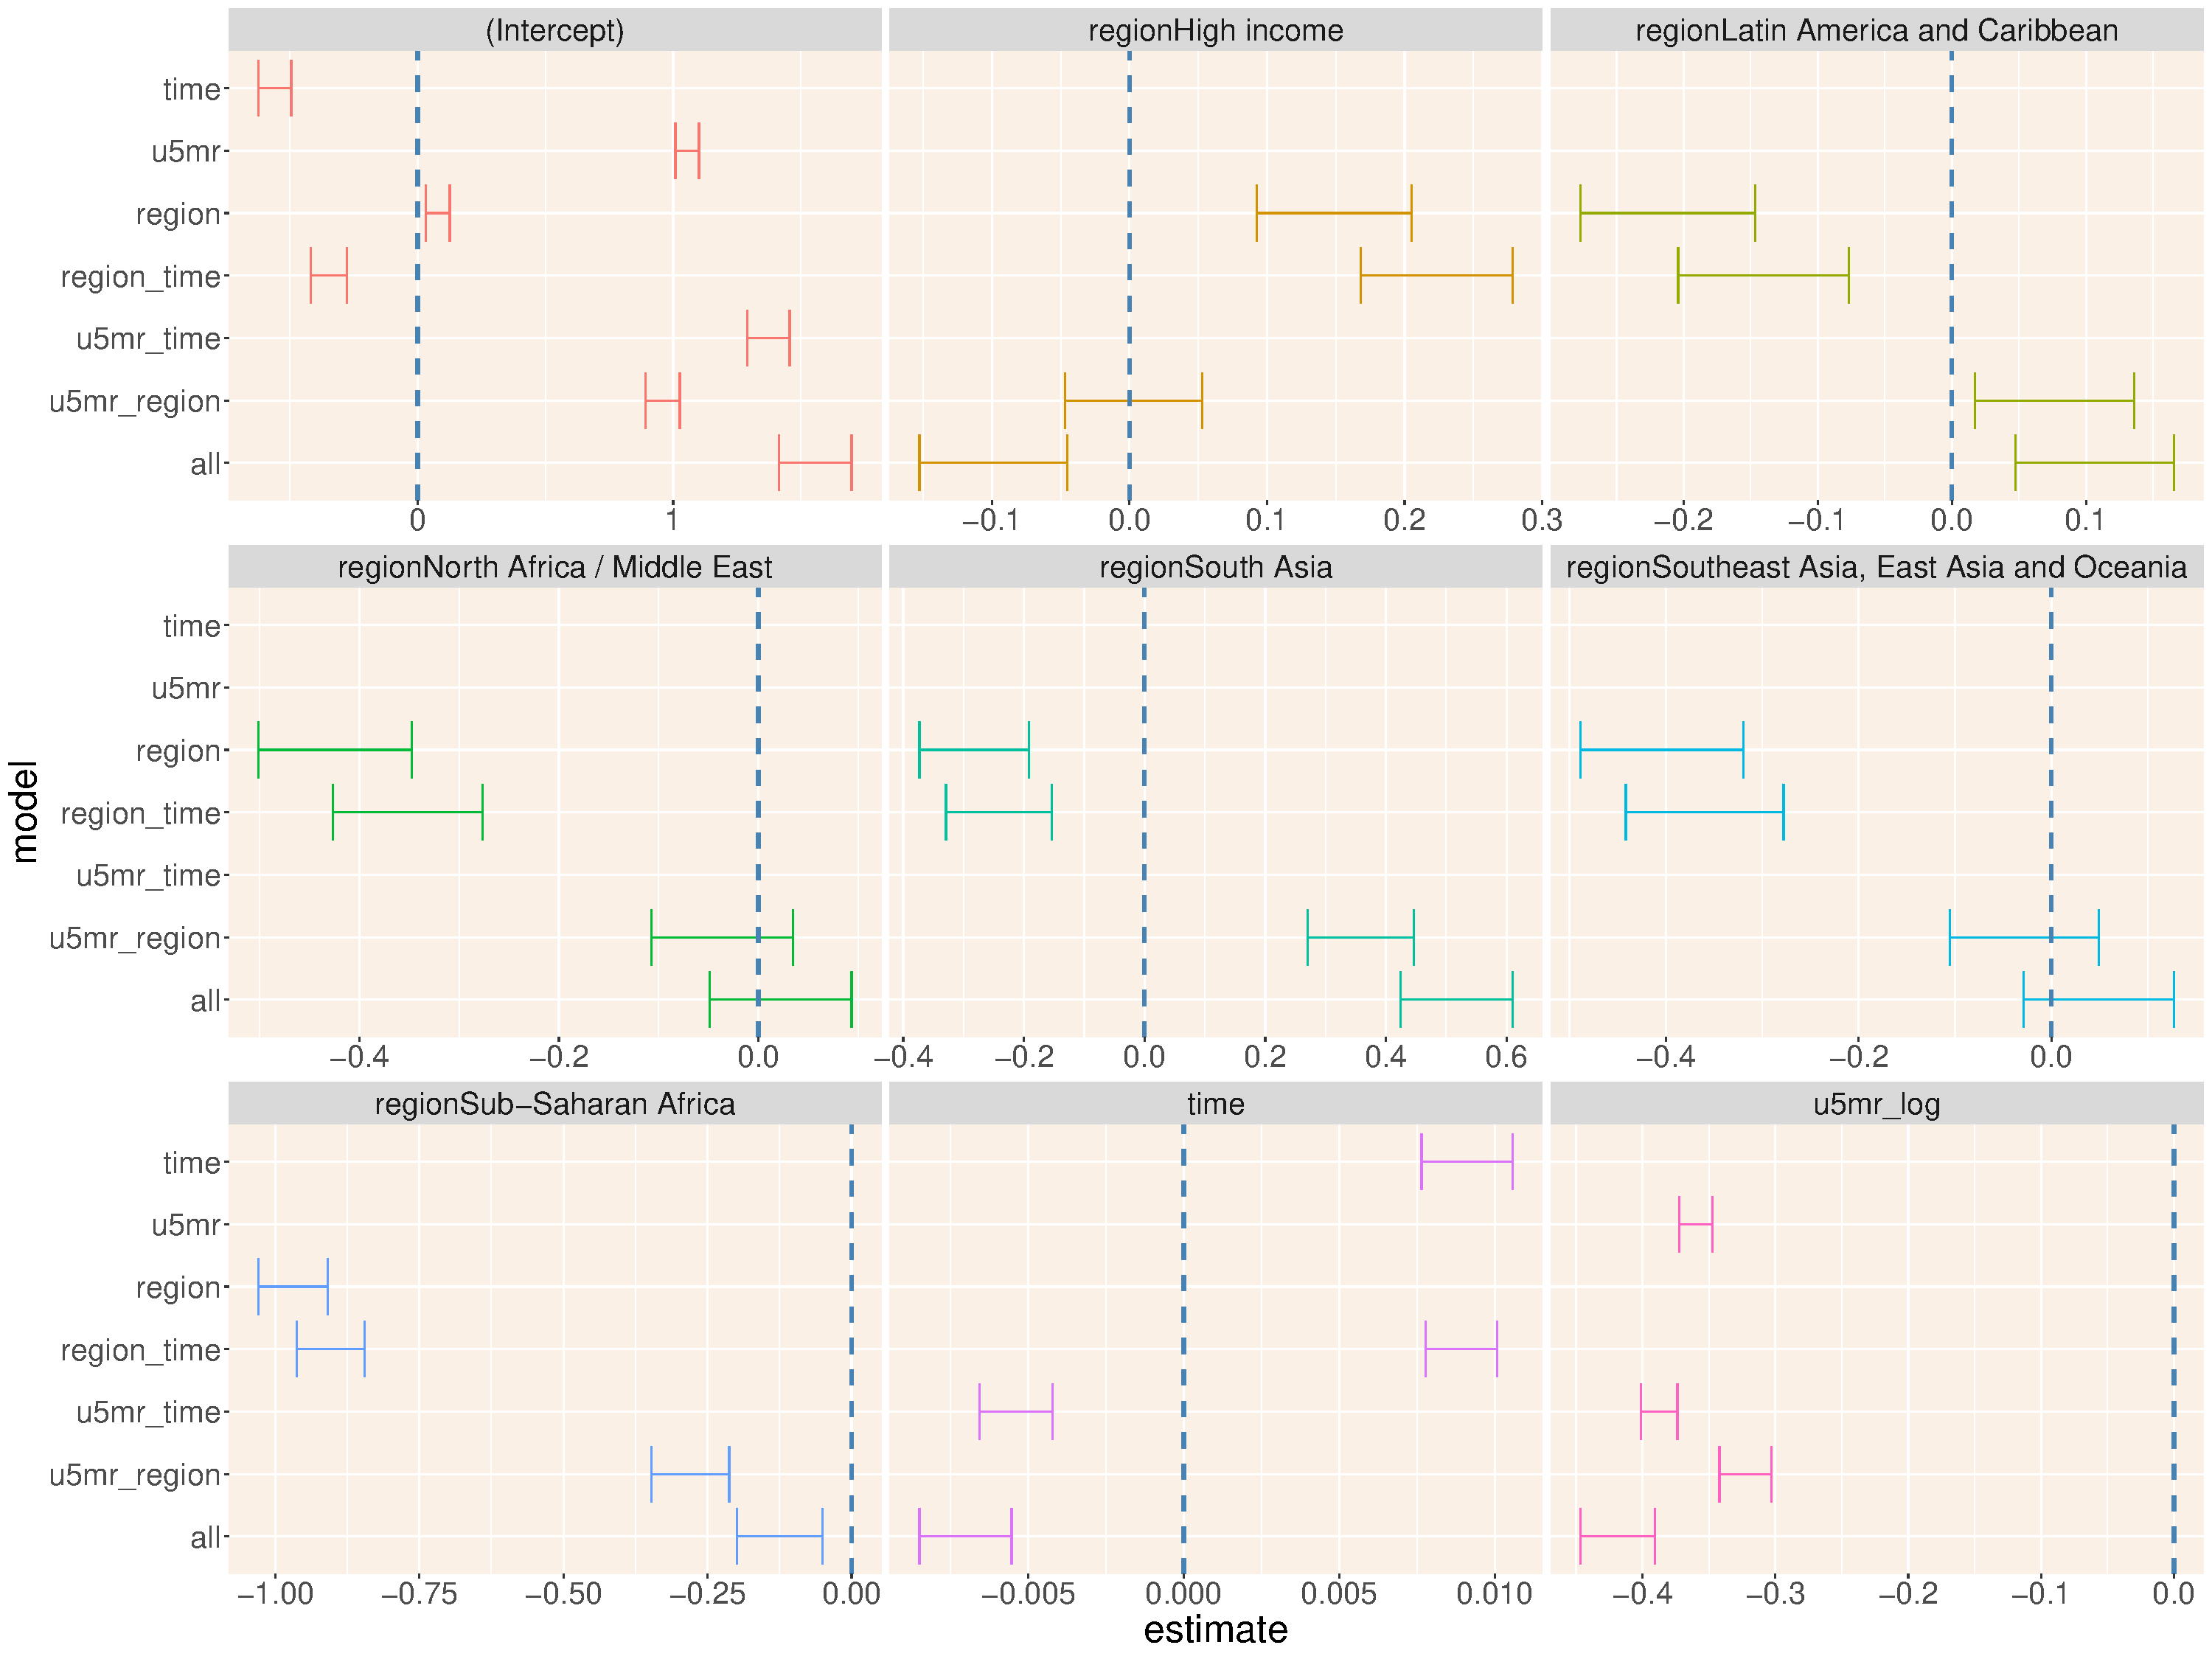
\includegraphics{A2_files/figure-latex/variable-choice-1.pdf}

In order to choose appropriate variables for the linear model, we have
created seven models which includes different variables. Then we fitted
seven different models into the error bar graph that represents the
significance of each variable in the model.

From the error bar we can see that the time variable is considered to be
significant among all models under the 95\% confidence interval, as both
the maximum and the minimum are different from 0. Similarly, variables
such as region, and u5mr can also be considered as significant. However,
while looking at the region\_time model which represents the interaction
effect between region and time, we can see that the shifts from the
region model are only significant for High income and Latin American
region; and therefore, the interaction effect should not be used here.

For u5mr\_region model, if we only consider u5mr or region, individually
they are significant. When region is conditional on u5mr, the variable
region turns from significant to insignificant, as it moves towards 0.
Therefore, u5mr will affect region, but region have no effect on u5mr.
We consider this is significant.

For u5mr\_time model, as we mentioned before, u5mr itself is
significant, while adding time, the significance level have not changed.
However, when it is conditional on u5mr, time have been affected from
positive values to negative significance values shown in graph t.
Therefore, time u5mr will affect time. We also consider this is
significant.

\begin{Shaded}
\begin{Highlighting}[]
\CommentTok{\# understanding relationship between the variables}
\FunctionTok{dagify}\NormalTok{(nmr }\SpecialCharTok{\textasciitilde{}}\NormalTok{ u5mr,}
\NormalTok{       nmr }\SpecialCharTok{\textasciitilde{}}\NormalTok{ time,}
\NormalTok{       nmr }\SpecialCharTok{\textasciitilde{}}\NormalTok{ Region,}
\NormalTok{       time }\SpecialCharTok{\textasciitilde{}}\NormalTok{ u5mr,}
\NormalTok{       Region }\SpecialCharTok{\textasciitilde{}}\NormalTok{ u5mr}
\NormalTok{       ) }\SpecialCharTok{\%\textgreater{}\%} 
  \FunctionTok{ggdag\_adjust}\NormalTok{(}\AttributeTok{node\_size =} \DecValTok{20}\NormalTok{) }\SpecialCharTok{+}
  \FunctionTok{theme\_dag}\NormalTok{(}\AttributeTok{legend.position =} \StringTok{"none"}\NormalTok{) }\SpecialCharTok{+}
  \FunctionTok{ggtitle}\NormalTok{(}\StringTok{"Relationship between the variables"}\NormalTok{) }\SpecialCharTok{+} 
  \FunctionTok{theme}\NormalTok{(}\AttributeTok{plot.title =} \FunctionTok{element\_text}\NormalTok{(}\AttributeTok{hjust =} \FloatTok{0.5}\NormalTok{))}
\end{Highlighting}
\end{Shaded}

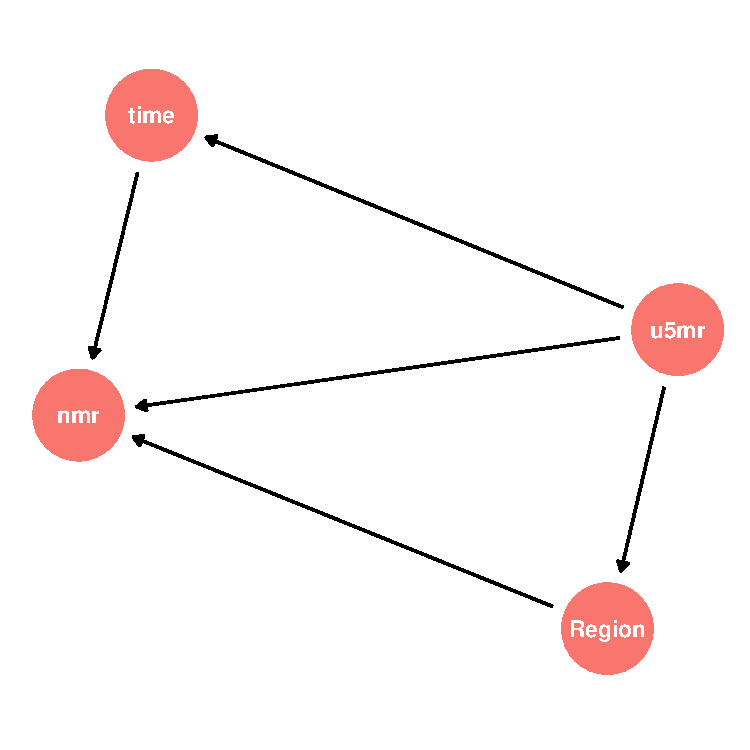
\includegraphics{A2_files/figure-latex/unnamed-chunk-3-1.pdf}

\begin{Shaded}
\begin{Highlighting}[]
\CommentTok{\# Fitting the model using the training data (with the interactive effect)}
\NormalTok{fit }\OtherTok{\textless{}{-}} \FunctionTok{lm}\NormalTok{(transformed\_nmr }\SpecialCharTok{\textasciitilde{}}\NormalTok{ u5mr\_log }\SpecialCharTok{+}\NormalTok{ u5mr\_log}\SpecialCharTok{*}\NormalTok{region }\SpecialCharTok{+}\NormalTok{ u5mr\_log}\SpecialCharTok{*}\NormalTok{time, nmr\_train)}

\FunctionTok{summary}\NormalTok{(fit)}
\end{Highlighting}
\end{Shaded}

\begin{verbatim}
## 
## Call:
## lm(formula = transformed_nmr ~ u5mr_log + u5mr_log * region + 
##     u5mr_log * time, data = nmr_train)
## 
## Residuals:
##     Min      1Q  Median      3Q     Max 
## -1.9753 -0.2320 -0.0115  0.2124  2.7544 
## 
## Coefficients:
##                                                       Estimate Std. Error
## (Intercept)                                           1.583037   0.128919
## u5mr_log                                             -0.423073   0.035458
## regionHigh income                                    -0.493517   0.076436
## regionLatin America and Caribbean                     0.824015   0.107731
## regionNorth Africa / Middle East                      0.374235   0.123906
## regionSouth Asia                                      1.339746   0.311316
## regionSoutheast Asia, East Asia and Oceania           0.630431   0.143342
## regionSub-Saharan Africa                              1.294305   0.143371
## time                                                 -0.012890   0.001864
## u5mr_log:regionHigh income                            0.180908   0.028745
## u5mr_log:regionLatin America and Caribbean           -0.227001   0.032338
## u5mr_log:regionNorth Africa / Middle East            -0.110263   0.034771
## u5mr_log:regionSouth Asia                            -0.215496   0.068215
## u5mr_log:regionSoutheast Asia, East Asia and Oceania -0.179566   0.039432
## u5mr_log:regionSub-Saharan Africa                    -0.334975   0.035098
## u5mr_log:time                                         0.002318   0.000458
##                                                      t value
## (Intercept)                                            12.28
## u5mr_log                                              -11.93
## regionHigh income                                      -6.46
## regionLatin America and Caribbean                       7.65
## regionNorth Africa / Middle East                        3.02
## regionSouth Asia                                        4.30
## regionSoutheast Asia, East Asia and Oceania             4.40
## regionSub-Saharan Africa                                9.03
## time                                                   -6.91
## u5mr_log:regionHigh income                              6.29
## u5mr_log:regionLatin America and Caribbean             -7.02
## u5mr_log:regionNorth Africa / Middle East              -3.17
## u5mr_log:regionSouth Asia                              -3.16
## u5mr_log:regionSoutheast Asia, East Asia and Oceania   -4.55
## u5mr_log:regionSub-Saharan Africa                      -9.54
## u5mr_log:time                                           5.06
##                                                                  Pr(>|t|)    
## (Intercept)                                          < 0.0000000000000002 ***
## u5mr_log                                             < 0.0000000000000002 ***
## regionHigh income                                       0.000000000122964 ***
## regionLatin America and Caribbean                       0.000000000000027 ***
## regionNorth Africa / Middle East                                   0.0025 ** 
## regionSouth Asia                                        0.000017306514550 ***
## regionSoutheast Asia, East Asia and Oceania             0.000011270533052 ***
## regionSub-Saharan Africa                             < 0.0000000000000002 ***
## time                                                    0.000000000005608 ***
## u5mr_log:regionHigh income                              0.000000000351939 ***
## u5mr_log:regionLatin America and Caribbean              0.000000000002693 ***
## u5mr_log:regionNorth Africa / Middle East                          0.0015 ** 
## u5mr_log:regionSouth Asia                                          0.0016 ** 
## u5mr_log:regionSoutheast Asia, East Asia and Oceania    0.000005461844858 ***
## u5mr_log:regionSub-Saharan Africa                    < 0.0000000000000002 ***
## u5mr_log:time                                           0.000000447100601 ***
## ---
## Signif. codes:  0 '***' 0.001 '**' 0.01 '*' 0.05 '.' 0.1 ' ' 1
## 
## Residual standard error: 0.41 on 3261 degrees of freedom
## Multiple R-squared:  0.615,  Adjusted R-squared:  0.613 
## F-statistic:  348 on 15 and 3261 DF,  p-value: <0.0000000000000002
\end{verbatim}

The dag graph illustrates The information about the relationship we get
from the error bar graph. The neonatal mortality rate (nmr) is the
dependent variable, from the dag graph we can see that both time and
region is piped. We do not want to add them, cause they will end up
worth less effect which removes the correlation between u5mr and nmr
because we are adding bias through time and region. u5mr is a fork
therefore we consider to include it. Moreover, from the error bar we see
the indirect affect to u5mr and time, therefore, to consider the
interaction effect, we include u5mr*region and u5mr*time.

\hypertarget{task-1.1.2-assess-your-linear-model-and-comment-on-its-fit.-this-should-be-done-a-for-all-data-simultaneously-bfor-data-in-each-region-and-c-for-data-in-a-maximum-of-3-countries-that-should-be-chosen-to-highlight-different-aspects-of-the-fit-diagnostics.}{%
\subsubsection{Task 1.1.2: Assess your linear model and comment on its
fit. This should be done a) for all data simultaneously; b)for data in
each region; and c) for data in a maximum of 3 countries that should be
chosen to highlight different aspects of the fit
diagnostics.}\label{task-1.1.2-assess-your-linear-model-and-comment-on-its-fit.-this-should-be-done-a-for-all-data-simultaneously-bfor-data-in-each-region-and-c-for-data-in-a-maximum-of-3-countries-that-should-be-chosen-to-highlight-different-aspects-of-the-fit-diagnostics.}}

\begin{Shaded}
\begin{Highlighting}[]
\NormalTok{augment\_fit }\OtherTok{\textless{}{-}}\NormalTok{ fit }\SpecialCharTok{\%\textgreater{}\%} 
  \FunctionTok{augment}\NormalTok{(}\AttributeTok{data =}\NormalTok{ nmr\_train)}
\CommentTok{\# Part a: For all data simultaneously}
\NormalTok{augment\_fit }\SpecialCharTok{\%\textgreater{}\%} 
  \FunctionTok{ggplot}\NormalTok{() }\SpecialCharTok{+}
  \FunctionTok{geom\_point}\NormalTok{(}\FunctionTok{aes}\NormalTok{(}\AttributeTok{x =}\NormalTok{ u5mr\_log, }\AttributeTok{y=}\NormalTok{ transformed\_nmr), }\AttributeTok{color =} \StringTok{"\#1b9ce3"}\NormalTok{)}\SpecialCharTok{+}
  \FunctionTok{geom\_line}\NormalTok{(}\FunctionTok{aes}\NormalTok{(}\AttributeTok{x =}\NormalTok{ u5mr\_log, }\AttributeTok{y =}\NormalTok{ .fitted), }\AttributeTok{color =} \StringTok{"\#ffda85"}\NormalTok{) }\SpecialCharTok{+}
  \FunctionTok{theme}\NormalTok{(}\AttributeTok{panel.background =} \FunctionTok{element\_rect}\NormalTok{(}\AttributeTok{fill =} \StringTok{"\#cae6da"}\NormalTok{), }\AttributeTok{text =} \FunctionTok{element\_text}\NormalTok{(}\AttributeTok{size=}\DecValTok{15}\NormalTok{),}
        \AttributeTok{plot.title =} \FunctionTok{element\_text}\NormalTok{(}\AttributeTok{hjust =} \FloatTok{0.5}\NormalTok{)) }\SpecialCharTok{+}
  \FunctionTok{xlab}\NormalTok{(}\StringTok{"Under 5 mortality rate in Log scale"}\NormalTok{) }\SpecialCharTok{+}
  \FunctionTok{ylab}\NormalTok{(}\StringTok{"Neonatal Mortality Rate in Log Scale"}\NormalTok{) }\SpecialCharTok{+}
  \FunctionTok{ggtitle}\NormalTok{(}\StringTok{"Linear model for all data simulatenously"}\NormalTok{)}
\end{Highlighting}
\end{Shaded}

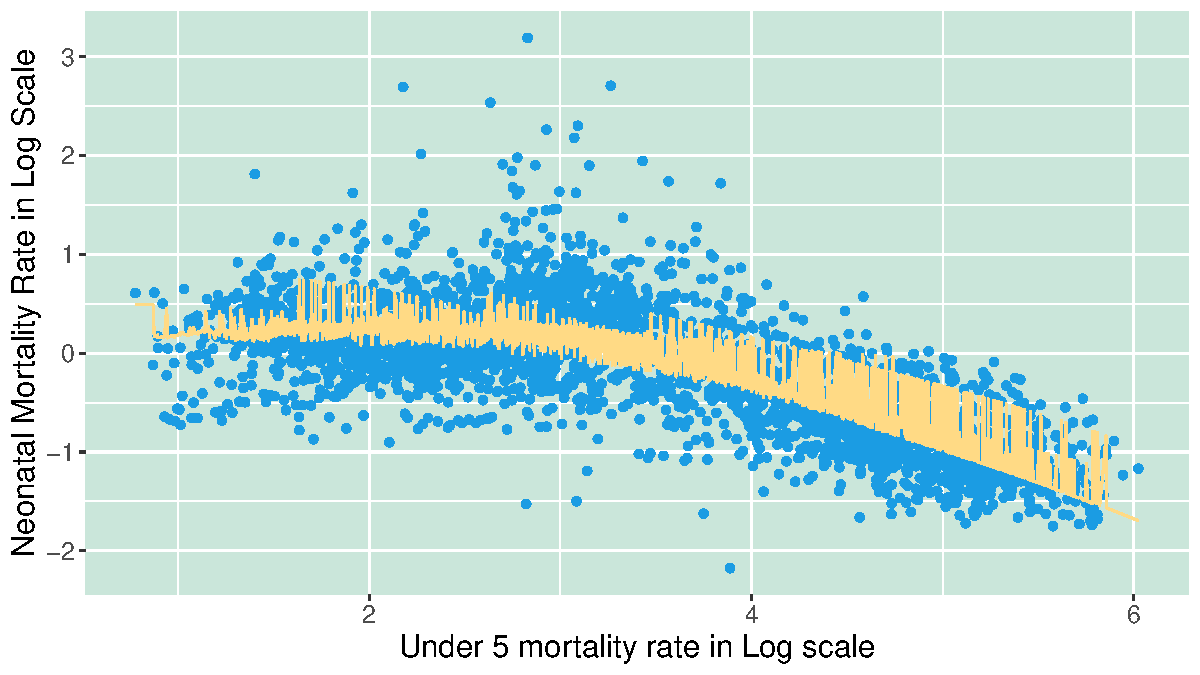
\includegraphics{A2_files/figure-latex/unnamed-chunk-4-1.pdf}

The fitted model fits fairly well with all the data simultaneously, as
we can see from the graph that the fitted model and the actual data
mostly overlap with each other.

\begin{Shaded}
\begin{Highlighting}[]
\NormalTok{augment\_fit }\SpecialCharTok{\%\textgreater{}\%} 
  \FunctionTok{ggplot}\NormalTok{(}\FunctionTok{aes}\NormalTok{(}\AttributeTok{sample=}\NormalTok{.resid}\SpecialCharTok{/}\NormalTok{.sigma)) }\SpecialCharTok{+}
  \FunctionTok{geom\_qq}\NormalTok{()}\SpecialCharTok{+}
  \FunctionTok{geom\_abline}\NormalTok{(}\AttributeTok{intercept=}\DecValTok{0}\NormalTok{, }\AttributeTok{slope =} \DecValTok{1}\NormalTok{) }\SpecialCharTok{+}
  \FunctionTok{theme}\NormalTok{(}\AttributeTok{panel.background =} \FunctionTok{element\_rect}\NormalTok{(}\AttributeTok{fill =} \StringTok{"\#cae6da"}\NormalTok{),}
        \AttributeTok{plot.title =} \FunctionTok{element\_text}\NormalTok{(}\AttributeTok{hjust =} \FloatTok{0.5}\NormalTok{)) }\SpecialCharTok{+}
  \FunctionTok{ggtitle}\NormalTok{(}\StringTok{"QQ Plot for all data"}\NormalTok{)}
\end{Highlighting}
\end{Shaded}

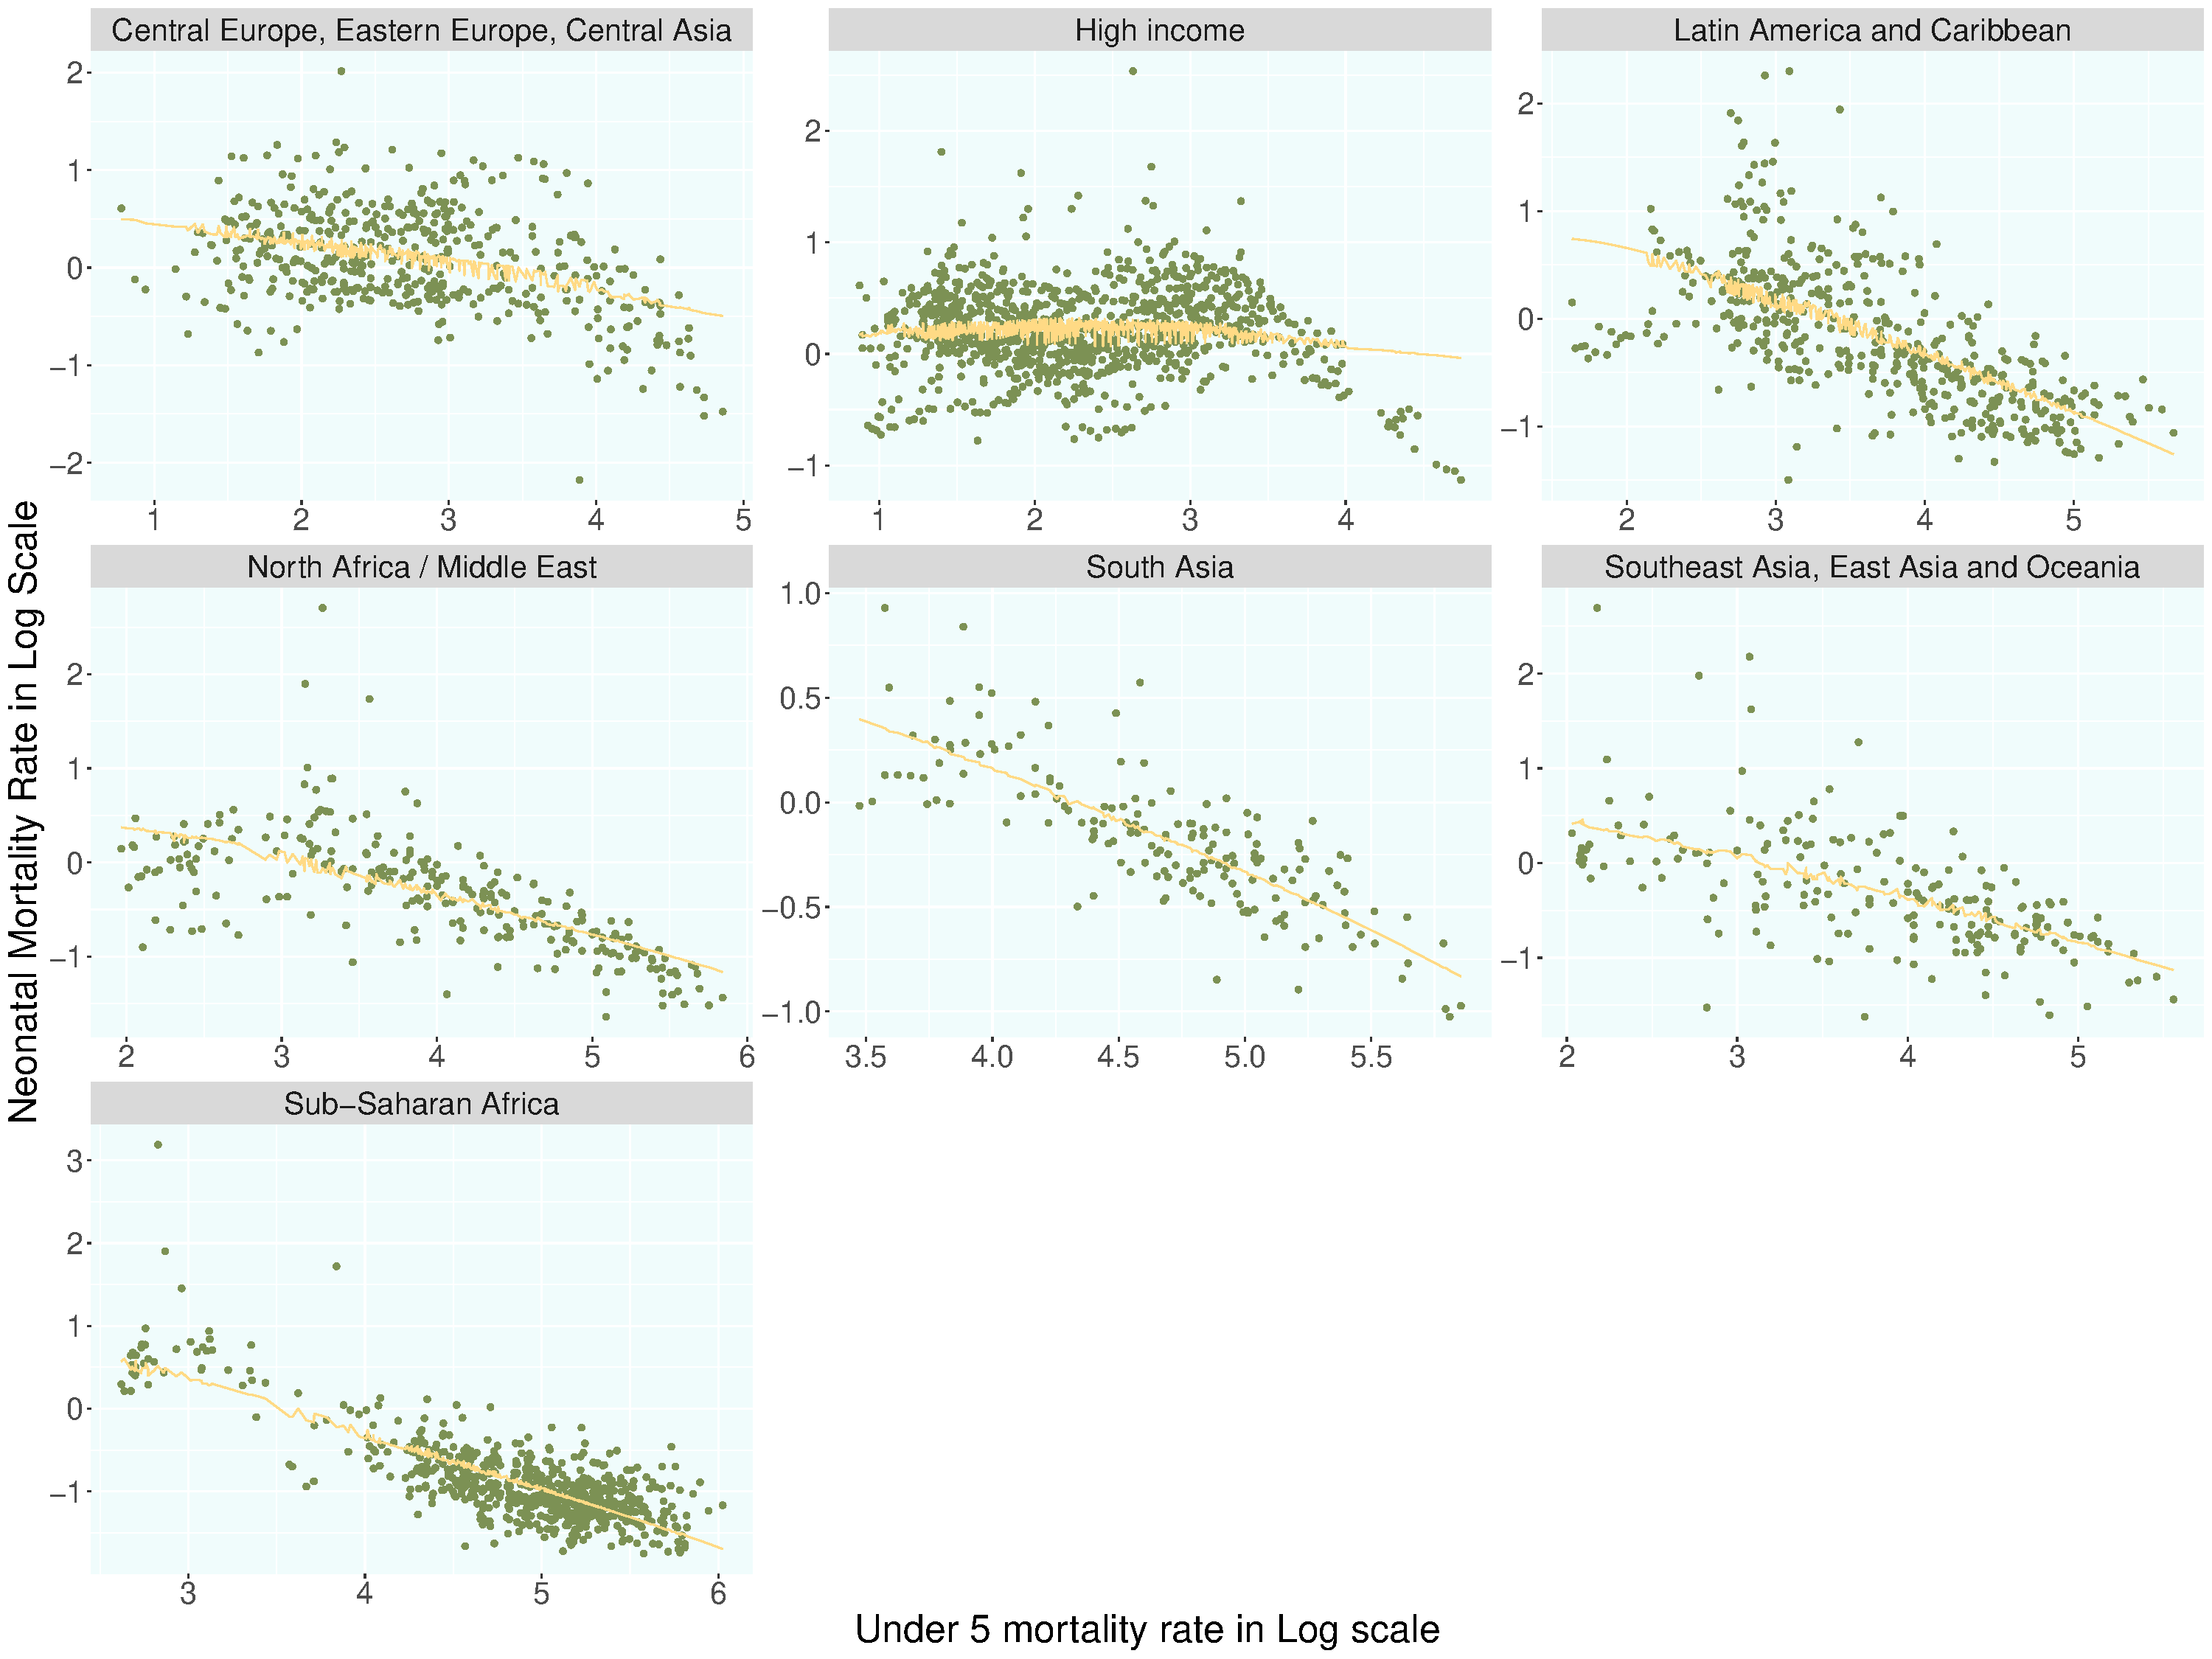
\includegraphics{A2_files/figure-latex/unnamed-chunk-5-1.pdf}

From the QQ-Plot, it can be observed that there is a heavy right tail
which is common in log scaled variables. The normality does not equal 1.

\begin{Shaded}
\begin{Highlighting}[]
\CommentTok{\# Part b: For data in each region}
\NormalTok{augment\_fit }\SpecialCharTok{\%\textgreater{}\%} 
  \FunctionTok{ggplot}\NormalTok{() }\SpecialCharTok{+}
  \FunctionTok{geom\_point}\NormalTok{(}\FunctionTok{aes}\NormalTok{(}\AttributeTok{x =}\NormalTok{ u5mr\_log, }\AttributeTok{y=}\NormalTok{ transformed\_nmr), }\AttributeTok{color =} \StringTok{"\#7c9154"}\NormalTok{)}\SpecialCharTok{+}
  \FunctionTok{geom\_line}\NormalTok{(}\FunctionTok{aes}\NormalTok{(}\AttributeTok{x =}\NormalTok{ u5mr\_log, }\AttributeTok{y =}\NormalTok{ .fitted), }\AttributeTok{color =} \StringTok{"\#ffda85"}\NormalTok{)}\SpecialCharTok{+}
  \FunctionTok{facet\_wrap}\NormalTok{(}\SpecialCharTok{\textasciitilde{}}\NormalTok{region, }\AttributeTok{scale =} \StringTok{"free"}\NormalTok{) }\SpecialCharTok{+}
  \FunctionTok{theme}\NormalTok{(}\AttributeTok{panel.background =} \FunctionTok{element\_rect}\NormalTok{(}\AttributeTok{fill =} \StringTok{"\#f0fcfc"}\NormalTok{), }\AttributeTok{text =} \FunctionTok{element\_text}\NormalTok{(}\AttributeTok{size=}\DecValTok{25}\NormalTok{),}
        \AttributeTok{plot.title =} \FunctionTok{element\_text}\NormalTok{(}\AttributeTok{hjust =} \FloatTok{0.5}\NormalTok{)) }\SpecialCharTok{+}
  \FunctionTok{xlab}\NormalTok{(}\StringTok{"Under 5 mortality rate in Log scale"}\NormalTok{) }\SpecialCharTok{+}
  \FunctionTok{ylab}\NormalTok{(}\StringTok{"Neonatal Mortality Rate in Log Scale"}\NormalTok{) }\SpecialCharTok{+}
  \FunctionTok{ggtitle}\NormalTok{(}\StringTok{"Linear model for each region"}\NormalTok{)}
\end{Highlighting}
\end{Shaded}

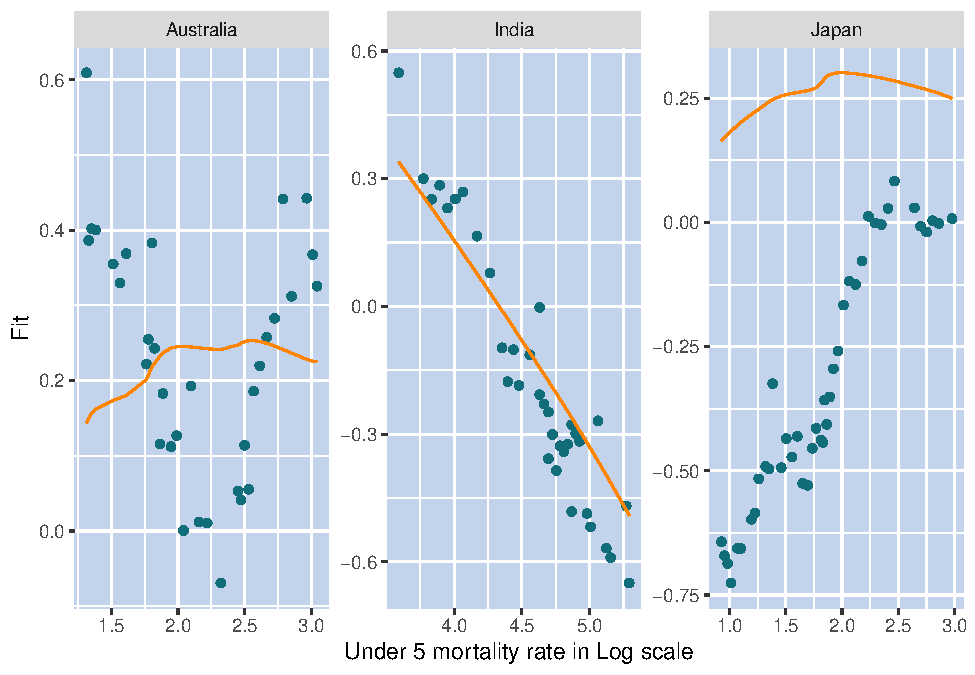
\includegraphics{A2_files/figure-latex/unnamed-chunk-6-1.pdf}

Similarly, the fitted model works well with data in each region as well,
especially for high income countries and Latin America and Caribbean.

\begin{Shaded}
\begin{Highlighting}[]
\NormalTok{augment\_fit }\SpecialCharTok{\%\textgreater{}\%} 
  \FunctionTok{ggplot}\NormalTok{(}\FunctionTok{aes}\NormalTok{(}\AttributeTok{sample=}\NormalTok{.resid}\SpecialCharTok{/}\NormalTok{.sigma)) }\SpecialCharTok{+}
  \FunctionTok{geom\_qq}\NormalTok{()}\SpecialCharTok{+}
  \FunctionTok{geom\_abline}\NormalTok{(}\AttributeTok{intercept=}\DecValTok{0}\NormalTok{, }\AttributeTok{slope =} \DecValTok{1}\NormalTok{) }\SpecialCharTok{+}
  \FunctionTok{facet\_wrap}\NormalTok{(}\SpecialCharTok{\textasciitilde{}}\NormalTok{region, }\AttributeTok{scale =} \StringTok{"free"}\NormalTok{) }\SpecialCharTok{+}
  \FunctionTok{theme}\NormalTok{(}\AttributeTok{panel.background =} \FunctionTok{element\_rect}\NormalTok{(}\AttributeTok{fill =} \StringTok{"\#f0fcfc"}\NormalTok{),}
        \AttributeTok{plot.title =} \FunctionTok{element\_text}\NormalTok{(}\AttributeTok{hjust =} \FloatTok{0.5}\NormalTok{)) }\SpecialCharTok{+}
  \FunctionTok{ggtitle}\NormalTok{(}\StringTok{"QQ Plot for each region"}\NormalTok{)}
\end{Highlighting}
\end{Shaded}

\includegraphics{A2_files/figure-latex/unnamed-chunk-7-1.pdf}

All regions except for South Asia, all other regions have a common
distribution.

\begin{Shaded}
\begin{Highlighting}[]
\CommentTok{\# Part c: For data in a maximum of 3 countries that should be chosen to highlight different aspects of the fit diagnostics}
\NormalTok{augment\_fit }\SpecialCharTok{\%\textgreater{}\%}
  \FunctionTok{filter}\NormalTok{(country\_name }\SpecialCharTok{\%in\%} \FunctionTok{c}\NormalTok{(}\StringTok{"India"}\NormalTok{, }\StringTok{"Japan"}\NormalTok{, }\StringTok{"Australia"}\NormalTok{)) }\SpecialCharTok{\%\textgreater{}\%}
  \FunctionTok{ggplot}\NormalTok{(}\FunctionTok{aes}\NormalTok{(}\AttributeTok{x =}\NormalTok{ u5mr\_log, }\AttributeTok{y =}\NormalTok{ transformed\_nmr)) }\SpecialCharTok{+}
  \FunctionTok{geom\_point}\NormalTok{(}\AttributeTok{color =} \StringTok{"\#126d7a"}\NormalTok{) }\SpecialCharTok{+}
  \FunctionTok{geom\_line}\NormalTok{(}\FunctionTok{aes}\NormalTok{(}\AttributeTok{x =}\NormalTok{ u5mr\_log, }\AttributeTok{y =}\NormalTok{ .fitted), }\AttributeTok{color =} \StringTok{"\#ff8400"}\NormalTok{) }\SpecialCharTok{+}
  \FunctionTok{facet\_wrap}\NormalTok{(}\SpecialCharTok{\textasciitilde{}}\NormalTok{country\_name, }\AttributeTok{scales =} \StringTok{"free"}\NormalTok{) }\SpecialCharTok{+}
  \FunctionTok{theme}\NormalTok{(}\AttributeTok{panel.background =} \FunctionTok{element\_rect}\NormalTok{(}\AttributeTok{fill =} \StringTok{"\#c3d3eb"}\NormalTok{),}
        \AttributeTok{plot.title =} \FunctionTok{element\_text}\NormalTok{(}\AttributeTok{hjust =} \FloatTok{0.5}\NormalTok{)) }\SpecialCharTok{+}
  \FunctionTok{xlab}\NormalTok{(}\StringTok{"Under 5 mortality rate in Log scale"}\NormalTok{) }\SpecialCharTok{+}
  \FunctionTok{ylab}\NormalTok{(}\StringTok{"Fit"}\NormalTok{) }\SpecialCharTok{+}
  \FunctionTok{ggtitle}\NormalTok{(}\StringTok{"Linear model for data in India, Japan and Australia"}\NormalTok{)}
\end{Highlighting}
\end{Shaded}

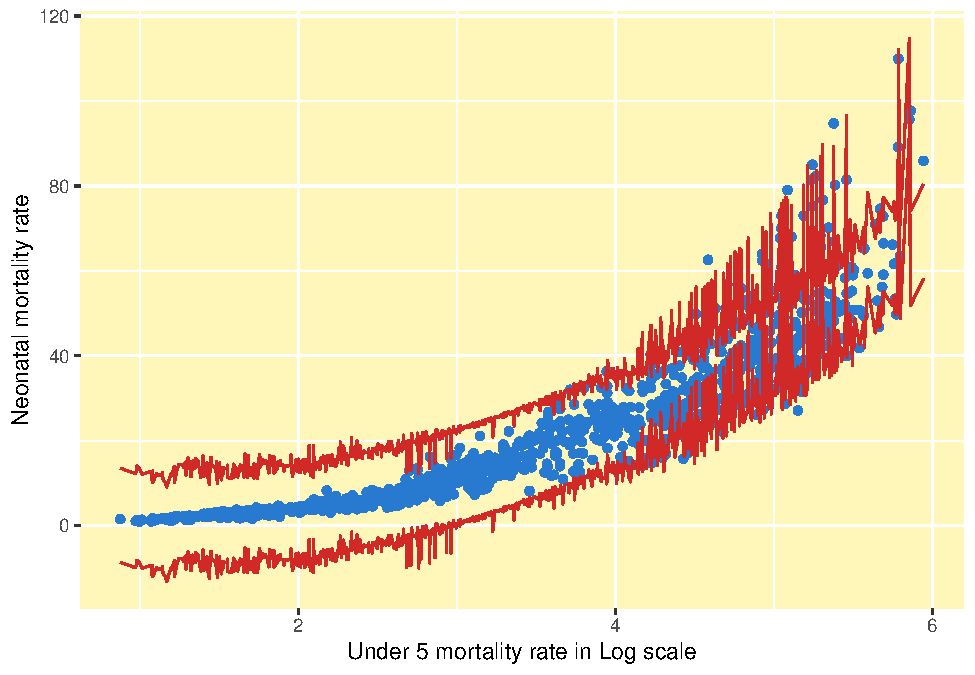
\includegraphics{A2_files/figure-latex/unnamed-chunk-8-1.pdf}

We choose India, Australia and Japan to highlight different aspects of
the fit. Australia and Japan both are developed countries, and India is
a developing country. For Australia and Japan, they fit terribly for the
model, especially Japan, none of the points are on the model. On
contrast, India fits better than the other two countries.

\begin{Shaded}
\begin{Highlighting}[]
\NormalTok{augment\_fit }\SpecialCharTok{\%\textgreater{}\%} 
  \FunctionTok{filter}\NormalTok{(country\_name }\SpecialCharTok{\%in\%} \FunctionTok{c}\NormalTok{(}\StringTok{"India"}\NormalTok{, }\StringTok{"Japan"}\NormalTok{, }\StringTok{"Australia"}\NormalTok{)) }\SpecialCharTok{\%\textgreater{}\%} 
  \FunctionTok{ggplot}\NormalTok{(}\FunctionTok{aes}\NormalTok{(}\AttributeTok{sample=}\NormalTok{.resid}\SpecialCharTok{/}\NormalTok{.sigma)) }\SpecialCharTok{+}
  \FunctionTok{geom\_qq}\NormalTok{()}\SpecialCharTok{+}
  \FunctionTok{geom\_abline}\NormalTok{(}\AttributeTok{intercept=}\DecValTok{0}\NormalTok{, }\AttributeTok{slope =} \DecValTok{1}\NormalTok{) }\SpecialCharTok{+}
  \FunctionTok{facet\_wrap}\NormalTok{(}\SpecialCharTok{\textasciitilde{}}\NormalTok{country\_name, }\AttributeTok{scales =} \StringTok{"free"}\NormalTok{) }\SpecialCharTok{+}
  \FunctionTok{theme}\NormalTok{(}\AttributeTok{panel.background =} \FunctionTok{element\_rect}\NormalTok{(}\AttributeTok{fill =} \StringTok{"\#f0fcfc"}\NormalTok{),}
        \AttributeTok{plot.title =} \FunctionTok{element\_text}\NormalTok{(}\AttributeTok{hjust =} \FloatTok{0.5}\NormalTok{)) }\SpecialCharTok{+}
  \FunctionTok{ggtitle}\NormalTok{(}\StringTok{"QQ Plot for India, Japan, Australia"}\NormalTok{)}
\end{Highlighting}
\end{Shaded}

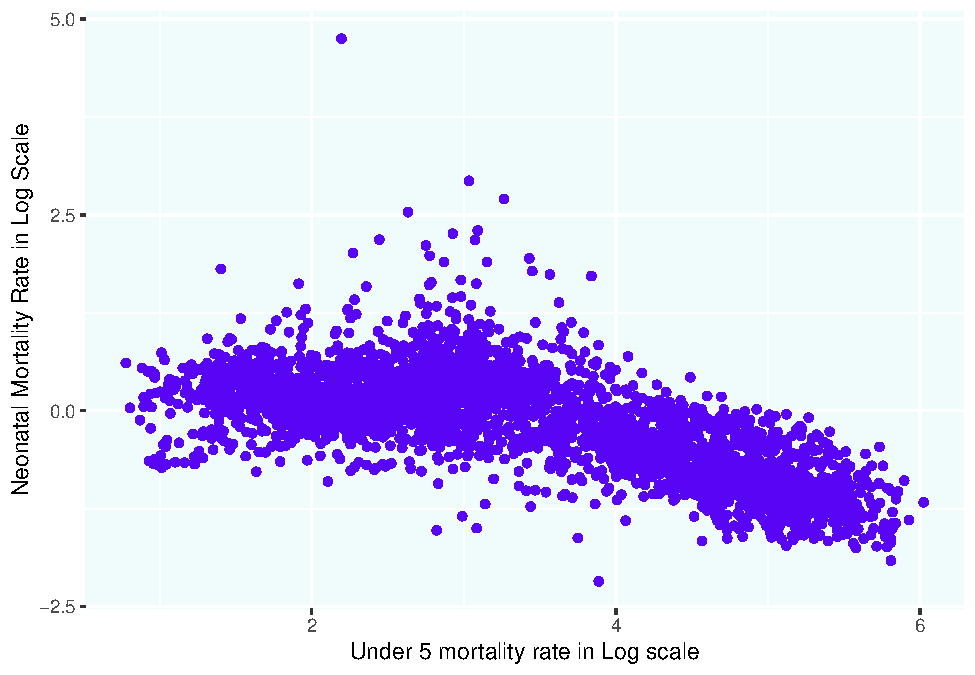
\includegraphics{A2_files/figure-latex/unnamed-chunk-9-1.pdf}

The QQ-Plot shows that none of the countries show a common distribution.

\hypertarget{task-1.1.3-estimate-the-root-mean-square-error-and-the-mean-absolute-error-on-a-test-set.-the-test-set-should-be-produced-using-the-argument-strata-region.}{%
\subsubsection{Task 1.1.3: Estimate the root mean square error and the
mean absolute error on a test set. The test set should be produced using
the argument strata =
region.}\label{task-1.1.3-estimate-the-root-mean-square-error-and-the-mean-absolute-error-on-a-test-set.-the-test-set-should-be-produced-using-the-argument-strata-region.}}

\begin{Shaded}
\begin{Highlighting}[]
\CommentTok{\# Predict the test dataset}
\NormalTok{lm\_pred }\OtherTok{\textless{}{-}} \FunctionTok{tibble}\NormalTok{(}\AttributeTok{pred =} \FunctionTok{predict}\NormalTok{(fit, nmr\_test))}
\NormalTok{lm\_pred }\OtherTok{\textless{}{-}} \FunctionTok{bind\_cols}\NormalTok{(nmr\_test, lm\_pred)}
\NormalTok{lm\_pred }\SpecialCharTok{\%\textgreater{}\%} 
  \FunctionTok{metrics}\NormalTok{(}\AttributeTok{truth =}\NormalTok{ transformed\_nmr,}
          \AttributeTok{estimate =}\NormalTok{ pred) }\SpecialCharTok{\%\textgreater{}\%} 
  \FunctionTok{kbl}\NormalTok{(}\AttributeTok{booktabs =}\NormalTok{ T,}
      \AttributeTok{caption =} \StringTok{"Mean absolute error, Root mean Square Error, R{-}squared value for the test set data"}\NormalTok{) }\SpecialCharTok{\%\textgreater{}\%}
  \FunctionTok{kable\_styling}\NormalTok{(}\AttributeTok{position =} \StringTok{"center"}\NormalTok{)}
\end{Highlighting}
\end{Shaded}

\begin{table}

\caption{\label{tab:unnamed-chunk-10}Mean absolute error, Root mean Square Error, R-squared value for the test set data}
\centering
\begin{tabular}[t]{llr}
\toprule
.metric & .estimator & .estimate\\
\midrule
rmse & standard & 0.43\\
rsq & standard & 0.59\\
mae & standard & 0.30\\
\bottomrule
\end{tabular}
\end{table}

According to Cornell Statistical Consulting Unit, RMSE is the square
root of the variance of the residuals, and ``It indicates the absolute
fit of the model to the data---how close the observed data points are to
the model's predicted values. (Grace-Martin, 2020) `` , and the lower
value of RMSE indicates the better fit of the model which the value we
have here is 0.4122092, meaning the difference between predicted value
and the observed value is a bit less than 50\%. Moreover, the r-squared
is 0.5986680, it means that the predicted model explains about 60\% of
the observed model. Additionally, MAE which stands for mean absolute
error measures the average magnitude of the errors in a set of
predictions, mae equals 0.3041219 meaning the errors between prediction
and actual observations are about 30\%.

\hypertarget{task-1.1.4-produce-a-prediction-with-prediction-intervals-of-the-nmr-on-its-natural-scale-aka-not-on-the-log-scale-and-plot-these-a-for-all-data-simultaneously-b-for-data-in-each-region-and-c-for-data-in-a-maximum-of-3-countries-that-show-different-aspects-of-the-fit.}{%
\subsubsection{Task 1.1.4: Produce a prediction, with prediction
intervals, of the NMR on its natural scale (aka not on the log-scale)
and plot these a) for all data simultaneously; b) for data in each
region; and c) for data in a maximum of 3 countries that show different
aspects of the
fit.}\label{task-1.1.4-produce-a-prediction-with-prediction-intervals-of-the-nmr-on-its-natural-scale-aka-not-on-the-log-scale-and-plot-these-a-for-all-data-simultaneously-b-for-data-in-each-region-and-c-for-data-in-a-maximum-of-3-countries-that-show-different-aspects-of-the-fit.}}

\begin{Shaded}
\begin{Highlighting}[]
\NormalTok{fit\_natural }\OtherTok{\textless{}{-}} \FunctionTok{lm}\NormalTok{(nmr }\SpecialCharTok{\textasciitilde{}}\NormalTok{ u5mr\_log }\SpecialCharTok{+}\NormalTok{ u5mr\_log}\SpecialCharTok{*}\NormalTok{region }\SpecialCharTok{+}\NormalTok{ u5mr\_log}\SpecialCharTok{*}\NormalTok{time, nmr\_train)}
\CommentTok{\# Prediction for all data simultaneously}
\NormalTok{linear\_prediction  }\OtherTok{\textless{}{-}} \FunctionTok{as\_tibble}\NormalTok{(}\FunctionTok{predict}\NormalTok{(fit\_natural, nmr\_test, }\AttributeTok{interval =} \StringTok{"prediction"}\NormalTok{)) }\SpecialCharTok{\%\textgreater{}\%} 
  \FunctionTok{bind\_cols}\NormalTok{(lm\_pred)}

\NormalTok{linear\_prediction  }\SpecialCharTok{\%\textgreater{}\%} 
  \FunctionTok{ggplot}\NormalTok{(}\FunctionTok{aes}\NormalTok{(}\AttributeTok{x =}\NormalTok{ u5mr\_log, }\AttributeTok{y =}\NormalTok{ nmr))}\SpecialCharTok{+}
  \FunctionTok{geom\_point}\NormalTok{(}\AttributeTok{color =} \StringTok{"\#287ad1"}\NormalTok{)}\SpecialCharTok{+}
  \FunctionTok{geom\_line}\NormalTok{(}\FunctionTok{aes}\NormalTok{(}\AttributeTok{y =}\NormalTok{ lwr), }\AttributeTok{color =} \StringTok{"\#d12828"}\NormalTok{)}\SpecialCharTok{+}
  \FunctionTok{geom\_line}\NormalTok{(}\FunctionTok{aes}\NormalTok{(}\AttributeTok{y =}\NormalTok{ upr), }\AttributeTok{color =} \StringTok{"\#d12828"}\NormalTok{) }\SpecialCharTok{+}
  \FunctionTok{theme}\NormalTok{(}\AttributeTok{panel.background =} \FunctionTok{element\_rect}\NormalTok{(}\AttributeTok{fill =} \StringTok{"\#fff6ba"}\NormalTok{),}
        \AttributeTok{plot.title =} \FunctionTok{element\_text}\NormalTok{(}\AttributeTok{hjust =} \FloatTok{0.5}\NormalTok{)) }\SpecialCharTok{+}
  \FunctionTok{xlab}\NormalTok{(}\StringTok{"Under 5 mortality rate in Log scale"}\NormalTok{) }\SpecialCharTok{+}
  \FunctionTok{ylab}\NormalTok{(}\StringTok{"Neonatal mortality rate"}\NormalTok{) }\SpecialCharTok{+}
  \FunctionTok{ggtitle}\NormalTok{(}\StringTok{"Prediction for all data simultaneously"}\NormalTok{)}
\end{Highlighting}
\end{Shaded}

\includegraphics{A2_files/figure-latex/unnamed-chunk-11-1.pdf}

Surprisingly, putting NMR on a natural scale does not look really
different from it is put on a log scale, only some values appear to be a
little bit extreme. However, putting upper and lower values exclude
these outliers.

\begin{Shaded}
\begin{Highlighting}[]
\CommentTok{\#  Prediction for region}
\NormalTok{linear\_prediction }\SpecialCharTok{\%\textgreater{}\%}
  \FunctionTok{ggplot}\NormalTok{(}\FunctionTok{aes}\NormalTok{(}\AttributeTok{x =}\NormalTok{ u5mr\_log, }\AttributeTok{y =}\NormalTok{ nmr))}\SpecialCharTok{+}
  \FunctionTok{geom\_point}\NormalTok{(}\AttributeTok{color =} \StringTok{"\#287ad1"}\NormalTok{)}\SpecialCharTok{+}
  \FunctionTok{geom\_line}\NormalTok{(}\FunctionTok{aes}\NormalTok{(}\AttributeTok{y =}\NormalTok{ lwr),}\AttributeTok{color =} \StringTok{"\#d12828"}\NormalTok{) }\SpecialCharTok{+}
  \FunctionTok{geom\_line}\NormalTok{(}\FunctionTok{aes}\NormalTok{(}\AttributeTok{y =}\NormalTok{ upr),}\AttributeTok{color =} \StringTok{"\#d12828"}\NormalTok{)}\SpecialCharTok{+}
  \FunctionTok{facet\_wrap}\NormalTok{(}\SpecialCharTok{\textasciitilde{}}\NormalTok{ region, }\AttributeTok{scale =} \StringTok{"free"}\NormalTok{)}\SpecialCharTok{+}
  \FunctionTok{theme}\NormalTok{(}\AttributeTok{panel.background =} \FunctionTok{element\_rect}\NormalTok{(}\AttributeTok{fill =} \StringTok{"\#fff6ba"}\NormalTok{),}
        \AttributeTok{plot.title =} \FunctionTok{element\_text}\NormalTok{(}\AttributeTok{hjust =} \FloatTok{0.5}\NormalTok{)) }\SpecialCharTok{+}
  \FunctionTok{xlab}\NormalTok{(}\StringTok{"Under 5 mortality rate in Log scale"}\NormalTok{) }\SpecialCharTok{+}
  \FunctionTok{ylab}\NormalTok{(}\StringTok{"Neonatal mortality rate"}\NormalTok{) }\SpecialCharTok{+}
  \FunctionTok{ggtitle}\NormalTok{(}\StringTok{"Prediction for each region"}\NormalTok{)}
\end{Highlighting}
\end{Shaded}

\includegraphics{A2_files/figure-latex/unnamed-chunk-12-1.pdf}

As for data in each region, Europe, High income countries, Latin America
and Caribbean and Sub-Saharan Africa, the lower and upper scales contain
most of the data, and the model performs well.

\begin{Shaded}
\begin{Highlighting}[]
\CommentTok{\#  Prediction for 3 Countires}
\NormalTok{ linear\_prediction }\SpecialCharTok{\%\textgreater{}\%}
  \FunctionTok{filter}\NormalTok{(country\_name }\SpecialCharTok{\%in\%} \FunctionTok{c}\NormalTok{(}\StringTok{"India"}\NormalTok{, }\StringTok{"Japan"}\NormalTok{, }\StringTok{"Australia"}\NormalTok{)) }\SpecialCharTok{\%\textgreater{}\%} 
  \FunctionTok{ggplot}\NormalTok{(}\FunctionTok{aes}\NormalTok{(}\AttributeTok{x =}\NormalTok{ u5mr\_log, }\AttributeTok{y =}\NormalTok{ nmr))}\SpecialCharTok{+}
  \FunctionTok{geom\_point}\NormalTok{(}\AttributeTok{color =} \StringTok{"\#287ad1"}\NormalTok{)}\SpecialCharTok{+}
  \FunctionTok{geom\_line}\NormalTok{(}\FunctionTok{aes}\NormalTok{(}\AttributeTok{y =}\NormalTok{ lwr), }\AttributeTok{color =} \StringTok{"\#d12828"}\NormalTok{) }\SpecialCharTok{+}
  \FunctionTok{geom\_line}\NormalTok{(}\FunctionTok{aes}\NormalTok{(}\AttributeTok{y =}\NormalTok{ upr), }\AttributeTok{color =} \StringTok{"\#d12828"}\NormalTok{)}\SpecialCharTok{+}
  \FunctionTok{facet\_wrap}\NormalTok{(}\SpecialCharTok{\textasciitilde{}}\NormalTok{ country\_name, }\AttributeTok{scale =} \StringTok{"free"}\NormalTok{)}\SpecialCharTok{+}
  \FunctionTok{theme}\NormalTok{(}\AttributeTok{panel.background =} \FunctionTok{element\_rect}\NormalTok{(}\AttributeTok{fill =} \StringTok{"\#fff6ba"}\NormalTok{),}
        \AttributeTok{plot.title =} \FunctionTok{element\_text}\NormalTok{(}\AttributeTok{hjust =} \FloatTok{0.5}\NormalTok{)) }\SpecialCharTok{+}
  \FunctionTok{xlab}\NormalTok{(}\StringTok{"Under 5 mortality rate in Log scale"}\NormalTok{) }\SpecialCharTok{+}
  \FunctionTok{ylab}\NormalTok{(}\StringTok{"Neonatal mortality rate"}\NormalTok{) }\SpecialCharTok{+}
  \FunctionTok{ggtitle}\NormalTok{(}\StringTok{"Prediction for India, Japan and Australia"}\NormalTok{)}
\end{Highlighting}
\end{Shaded}

\includegraphics{A2_files/figure-latex/unnamed-chunk-13-1.pdf}

As for the countries, Australia, India and Japan, putting upper and
lower scales looks like a better idea than the fit in the log scale,
while for Japan, some outliers are still excluded.

\hypertarget{task-1.2-non-linear-regression}{%
\subsection{Task 1.2: Non-linear
Regression}\label{task-1.2-non-linear-regression}}

\hypertarget{task-1.2.1-explain-your-choice-of-model-using-appropriate-visualisations-to-support-your-choice.}{%
\subsubsection{Task 1.2.1: Explain your choice of model, using
appropriate visualisations to support your
choice.}\label{task-1.2.1-explain-your-choice-of-model-using-appropriate-visualisations-to-support-your-choice.}}

\begin{Shaded}
\begin{Highlighting}[]
\CommentTok{\#non{-}linear variable}

\CommentTok{\#non{-}linear variable part1 choose variable}


\CommentTok{\# find which variables have non{-}linear relationship}
\CommentTok{\#u5mr\_log and transformed\_nmr non linear relationship}
\FunctionTok{ggplot}\NormalTok{(nmr\_train)}\SpecialCharTok{+}
  \FunctionTok{geom\_point}\NormalTok{(}\FunctionTok{aes}\NormalTok{(}\AttributeTok{x =}\NormalTok{ u5mr\_log, }\AttributeTok{y =}\NormalTok{ transformed\_nmr), }\AttributeTok{color =} \StringTok{"\#5905f5"}\NormalTok{)}\SpecialCharTok{+}
  \FunctionTok{theme}\NormalTok{(}\AttributeTok{panel.background =} \FunctionTok{element\_rect}\NormalTok{(}\AttributeTok{fill =} \StringTok{"\#f0fcfc"}\NormalTok{),}
        \AttributeTok{plot.title =} \FunctionTok{element\_text}\NormalTok{(}\AttributeTok{hjust =} \FloatTok{0.5}\NormalTok{)) }\SpecialCharTok{+}
  \FunctionTok{xlab}\NormalTok{(}\StringTok{"Under 5 mortality rate in Log scale"}\NormalTok{) }\SpecialCharTok{+}
  \FunctionTok{ylab}\NormalTok{(}\StringTok{"Neonatal Mortality Rate in Log Scale"}\NormalTok{) }\SpecialCharTok{+}
  \FunctionTok{ggtitle}\NormalTok{(}\StringTok{"u5mr\_log vs transformed\_nmr"}\NormalTok{)}
\end{Highlighting}
\end{Shaded}

\includegraphics{A2_files/figure-latex/unnamed-chunk-14-1.pdf}

\begin{Shaded}
\begin{Highlighting}[]
\CommentTok{\#time and transformed\_nmr, no non{-}linear relationship}
\FunctionTok{ggplot}\NormalTok{(nmr\_train)}\SpecialCharTok{+}
  \FunctionTok{geom\_point}\NormalTok{(}\FunctionTok{aes}\NormalTok{(}\AttributeTok{x =}\NormalTok{ time, }\AttributeTok{y =}\NormalTok{ transformed\_nmr), }\AttributeTok{color =} \StringTok{"\#5905f5"}\NormalTok{)}\SpecialCharTok{+}
  \FunctionTok{theme}\NormalTok{(}\AttributeTok{panel.background =} \FunctionTok{element\_rect}\NormalTok{(}\AttributeTok{fill =} \StringTok{"\#f0fcfc"}\NormalTok{),}
        \AttributeTok{plot.title =} \FunctionTok{element\_text}\NormalTok{(}\AttributeTok{hjust =} \FloatTok{0.5}\NormalTok{)) }\SpecialCharTok{+}
  \FunctionTok{xlab}\NormalTok{(}\StringTok{"Years"}\NormalTok{) }\SpecialCharTok{+}
  \FunctionTok{ylab}\NormalTok{(}\StringTok{"Neonatal Mortality Rate in Log Scale"}\NormalTok{)}\SpecialCharTok{+}
  \FunctionTok{ggtitle}\NormalTok{(}\StringTok{"Time vs transformed\_nmr"}\NormalTok{)}
\end{Highlighting}
\end{Shaded}

\includegraphics{A2_files/figure-latex/unnamed-chunk-14-2.pdf}

\begin{Shaded}
\begin{Highlighting}[]
\CommentTok{\#region and transformed\_nmr, no non{-}linear}
\FunctionTok{ggplot}\NormalTok{(nmr\_train)}\SpecialCharTok{+}
  \FunctionTok{geom\_point}\NormalTok{(}\FunctionTok{aes}\NormalTok{(}\AttributeTok{y =}\NormalTok{ region, }\AttributeTok{x =}\NormalTok{ transformed\_nmr), }\AttributeTok{color =} \StringTok{"\#5905f5"}\NormalTok{)}\SpecialCharTok{+}
  \FunctionTok{theme}\NormalTok{(}\AttributeTok{panel.background =} \FunctionTok{element\_rect}\NormalTok{(}\AttributeTok{fill =} \StringTok{"\#f0fcfc"}\NormalTok{),}
        \AttributeTok{plot.title =} \FunctionTok{element\_text}\NormalTok{(}\AttributeTok{hjust =} \FloatTok{0.5}\NormalTok{)) }\SpecialCharTok{+}
  \FunctionTok{ylab}\NormalTok{(}\StringTok{"Region"}\NormalTok{) }\SpecialCharTok{+}
  \FunctionTok{xlab}\NormalTok{(}\StringTok{"Neonatal Mortality Rate in Log Scale"}\NormalTok{) }\SpecialCharTok{+}
  \FunctionTok{ggtitle}\NormalTok{(}\StringTok{"Region vs transformed\_nmr"}\NormalTok{)}
\end{Highlighting}
\end{Shaded}

\includegraphics{A2_files/figure-latex/unnamed-chunk-14-3.pdf}

We first look for the variables with non-linear relationship. The first
graph is u5mr\_log and transformed\_nmr, the second graph is time and
transformed\_nmr, the third is region and transformed\_nmr, and it
appears that only u5mr\_log and transformed\_nmr has non-linear
relationship. We then fit a model with u5mr\_log, u5mr\_log*region and
u5mr\_log*time.

\hypertarget{task-1.2.2-use-cross-validation-to-select-an-appropriate-number-of-basis-functions-for-bs}{%
\subsubsection{Task 1.2.2: Use cross-validation to select an appropriate
number of basis functions for
bs()}\label{task-1.2.2-use-cross-validation-to-select-an-appropriate-number-of-basis-functions-for-bs}}

We use folds to split the data into groups.

\begin{Shaded}
\begin{Highlighting}[]
\CommentTok{\# non{-}linear model}
\NormalTok{fit\_non\_linear }\OtherTok{\textless{}{-}} \FunctionTok{lm}\NormalTok{(transformed\_nmr }\SpecialCharTok{\textasciitilde{}} \FunctionTok{bs}\NormalTok{(u5mr\_log, }\AttributeTok{df=} \DecValTok{15}\NormalTok{) }\SpecialCharTok{+}\NormalTok{ u5mr\_log}\SpecialCharTok{*}\NormalTok{region }\SpecialCharTok{+}\NormalTok{ u5mr\_log}\SpecialCharTok{*}\NormalTok{time, }\AttributeTok{data =}\NormalTok{ nmr\_train)}

\CommentTok{\#fold data into groups}
\NormalTok{folds }\OtherTok{\textless{}{-}} \FunctionTok{vfold\_cv}\NormalTok{(nmr\_data , }\AttributeTok{v =} \DecValTok{20}\NormalTok{, }\AttributeTok{strata =}\NormalTok{ region)}

\CommentTok{\# create recipe}
\NormalTok{bs\_recipe }\OtherTok{\textless{}{-}} \FunctionTok{recipe}\NormalTok{(transformed\_nmr }\SpecialCharTok{\textasciitilde{}}\NormalTok{ u5mr\_log }\SpecialCharTok{+}\NormalTok{ region }\SpecialCharTok{+}\NormalTok{ time,}
              \AttributeTok{data =}\NormalTok{ nmr\_train) }\SpecialCharTok{\%\textgreater{}\%} 
  \FunctionTok{step\_bs}\NormalTok{(u5mr\_log, }\AttributeTok{deg\_free =} \FunctionTok{tune}\NormalTok{()) }\SpecialCharTok{\%\textgreater{}\%} 
  \FunctionTok{step\_dummy}\NormalTok{(region) }\SpecialCharTok{\%\textgreater{}\%} 
  \FunctionTok{step\_interact}\NormalTok{(}\SpecialCharTok{\textasciitilde{}}\FunctionTok{starts\_with}\NormalTok{(}\StringTok{"u5mr\_log"}\NormalTok{)}\SpecialCharTok{:}\FunctionTok{starts\_with}\NormalTok{(}\StringTok{"region"}\NormalTok{))}

\CommentTok{\# add recipe to the workflow}
\NormalTok{wf\_bs }\OtherTok{\textless{}{-}} \FunctionTok{workflow}\NormalTok{() }\SpecialCharTok{\%\textgreater{}\%}
  \FunctionTok{add\_recipe}\NormalTok{(bs\_recipe)}

\CommentTok{\# create spec}
\NormalTok{spec }\OtherTok{\textless{}{-}} \FunctionTok{linear\_reg}\NormalTok{() }\SpecialCharTok{\%\textgreater{}\%}
  \FunctionTok{set\_engine}\NormalTok{(}\StringTok{"lm"}\NormalTok{)}


\NormalTok{wf\_lm }\OtherTok{\textless{}{-}}\NormalTok{ wf\_bs }\SpecialCharTok{\%\textgreater{}\%} 
  \FunctionTok{add\_model}\NormalTok{(spec) }

\NormalTok{fit\_lm }\OtherTok{\textless{}{-}}\NormalTok{ wf\_lm }\SpecialCharTok{\%\textgreater{}\%}
  \FunctionTok{tune\_grid}\NormalTok{(}\AttributeTok{resamples =}\NormalTok{ folds)}
\end{Highlighting}
\end{Shaded}

\begin{Shaded}
\begin{Highlighting}[]
\NormalTok{lowest\_rmse }\OtherTok{\textless{}{-}}\NormalTok{ fit\_lm }\SpecialCharTok{\%\textgreater{}\%} 
  \FunctionTok{select\_best}\NormalTok{(}\StringTok{"rmse"}\NormalTok{)}

\NormalTok{lowest\_rmse }\SpecialCharTok{\%\textgreater{}\%}\NormalTok{ knitr}\SpecialCharTok{::}\FunctionTok{kable}\NormalTok{()}
\end{Highlighting}
\end{Shaded}

\begin{tabular}{r|l}
\hline
deg\_free & .config\\
\hline
9 & Preprocessor05\_Model1\\
\hline
\end{tabular}

We used cross-validation to select an appropriate number of basis
functions for bs(), we first split the data into groups by folds, then
create recipes and add it to the workflow. In addition, we set up a spec
to discover the value of lambda with the smallest average root square
error.From the visualization of the error bar we find the lowest root
mean square error to select the degree of freedom to be 8.

\hypertarget{task-1.2.3-for-your-final-model-assess-your-linear-model-and-comment-on-its-fit.-this-should-be-done-a-for-all-data-simultaneously-b-for-data-in-each-region-and-c-for-data-in-a-maximum-of-3-countries-that-should-be-chosen-to-highlight-different-aspects-of-the-fit-diagnostics.}{%
\subsubsection{Task 1.2.3: For your final model, assess your linear
model and comment on its fit. This should be done a) for all data
simultaneously; b) for data in each region; and c) for data in a maximum
of 3 countries that should be chosen to highlight different aspects of
the fit
diagnostics.}\label{task-1.2.3-for-your-final-model-assess-your-linear-model-and-comment-on-its-fit.-this-should-be-done-a-for-all-data-simultaneously-b-for-data-in-each-region-and-c-for-data-in-a-maximum-of-3-countries-that-should-be-chosen-to-highlight-different-aspects-of-the-fit-diagnostics.}}

\begin{Shaded}
\begin{Highlighting}[]
\CommentTok{\# non{-}linear all}
\NormalTok{augment\_non\_linear }\OtherTok{\textless{}{-}}\NormalTok{ fit\_non\_linear }\SpecialCharTok{\%\textgreater{}\%} 
  \FunctionTok{augment}\NormalTok{(}\AttributeTok{data =}\NormalTok{ nmr\_train) }


\NormalTok{augment\_non\_linear }\SpecialCharTok{\%\textgreater{}\%} 
  \FunctionTok{ggplot}\NormalTok{(}\FunctionTok{aes}\NormalTok{(}\AttributeTok{x =}\NormalTok{ u5mr\_log, }\AttributeTok{y =}\NormalTok{ transformed\_nmr)) }\SpecialCharTok{+}
  \FunctionTok{geom\_point}\NormalTok{()}\SpecialCharTok{+}
  \FunctionTok{geom\_line}\NormalTok{(}\FunctionTok{aes}\NormalTok{(}\AttributeTok{x =}\NormalTok{ u5mr\_log, }\AttributeTok{y =}\NormalTok{ .fitted), }\AttributeTok{color =} \StringTok{"blue"}\NormalTok{)}\SpecialCharTok{+}
  \FunctionTok{theme}\NormalTok{(}\AttributeTok{panel.background =} \FunctionTok{element\_rect}\NormalTok{(}\AttributeTok{fill =} \StringTok{"\#f0fcfc"}\NormalTok{),}
        \AttributeTok{plot.title =} \FunctionTok{element\_text}\NormalTok{(}\AttributeTok{hjust =} \FloatTok{0.5}\NormalTok{)) }\SpecialCharTok{+}
  \FunctionTok{ggtitle}\NormalTok{(}\StringTok{"Non{-}linear model for all data simultaneously"}\NormalTok{)}
\end{Highlighting}
\end{Shaded}

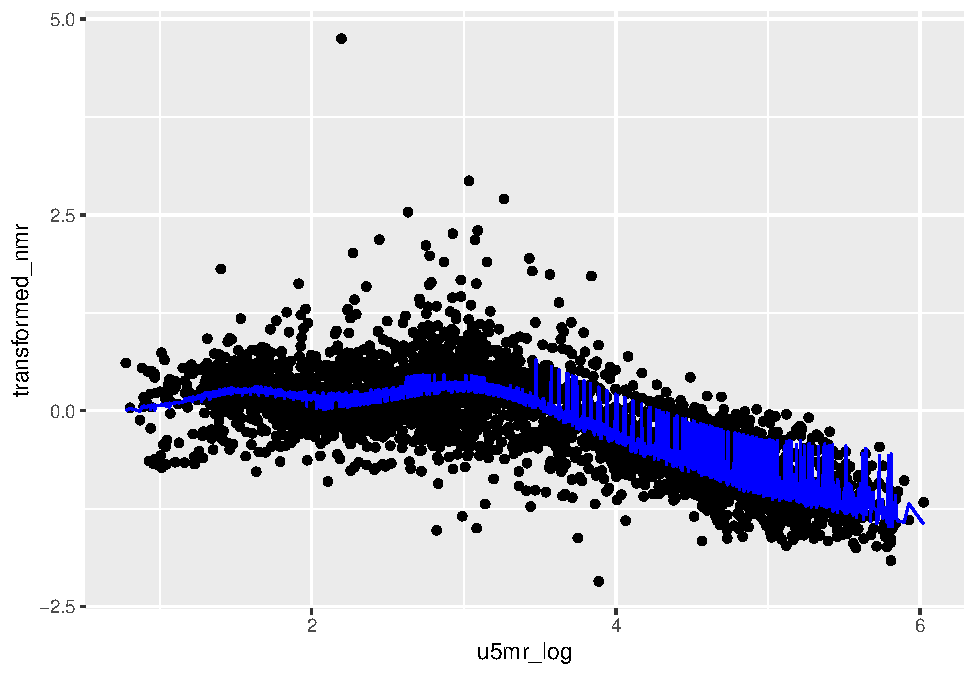
\includegraphics{A2_files/figure-latex/unnamed-chunk-17-1.pdf}

\begin{Shaded}
\begin{Highlighting}[]
\NormalTok{augment\_non\_linear }\SpecialCharTok{\%\textgreater{}\%} 
  \FunctionTok{ggplot}\NormalTok{(}\FunctionTok{aes}\NormalTok{(}\AttributeTok{sample=}\NormalTok{.resid}\SpecialCharTok{/}\NormalTok{.sigma)) }\SpecialCharTok{+}
  \FunctionTok{geom\_qq}\NormalTok{()}\SpecialCharTok{+}
  \FunctionTok{geom\_abline}\NormalTok{(}\AttributeTok{intercept=}\DecValTok{0}\NormalTok{, }\AttributeTok{slope =} \DecValTok{1}\NormalTok{) }\SpecialCharTok{+}
  \FunctionTok{theme}\NormalTok{(}\AttributeTok{panel.background =} \FunctionTok{element\_rect}\NormalTok{(}\AttributeTok{fill =} \StringTok{"\#f0fcfc"}\NormalTok{),}
        \AttributeTok{plot.title =} \FunctionTok{element\_text}\NormalTok{(}\AttributeTok{hjust =} \FloatTok{0.5}\NormalTok{)) }\SpecialCharTok{+}
  \FunctionTok{ggtitle}\NormalTok{(}\StringTok{"QQ Plot for all data in non{-}linear model"}\NormalTok{)}
\end{Highlighting}
\end{Shaded}

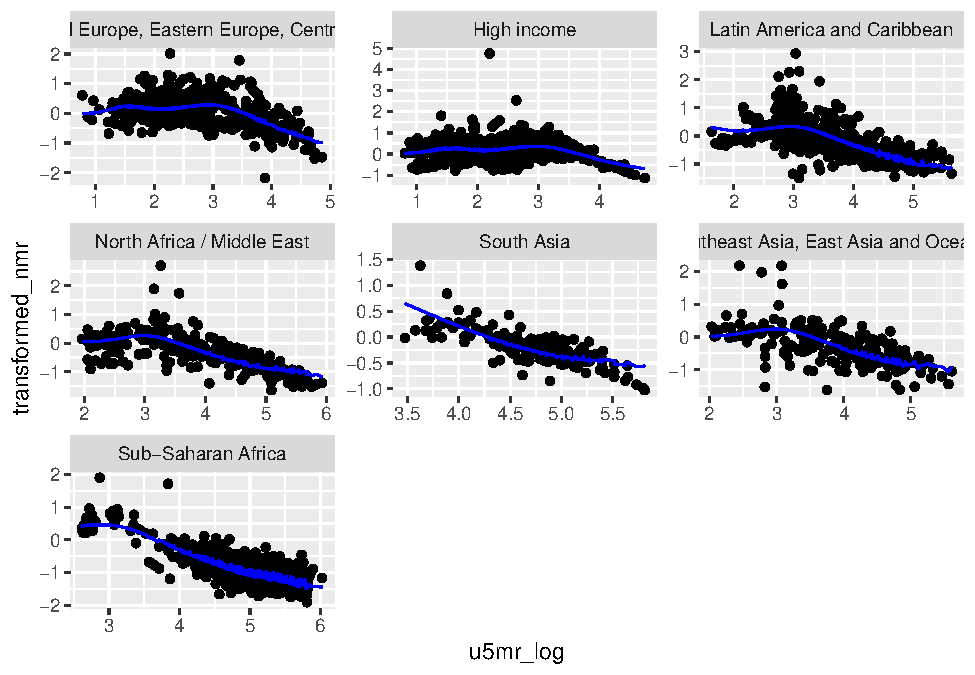
\includegraphics{A2_files/figure-latex/unnamed-chunk-17-2.pdf}

For the non-linear model, fitting the whole data simultaneously looks
really similar to the linear model, both of them are good fit. Since the
tails in QQ-Plot are not overlapping with the line, it indicates that
the data has more extreme values than the values that would be obtained
from a normal distribution.

\begin{Shaded}
\begin{Highlighting}[]
\CommentTok{\#non{-} linear region}
\NormalTok{augment\_non\_linear }\SpecialCharTok{\%\textgreater{}\%} 
  \FunctionTok{ggplot}\NormalTok{(}\FunctionTok{aes}\NormalTok{(}\AttributeTok{x =}\NormalTok{ u5mr\_log, }\AttributeTok{y =}\NormalTok{ transformed\_nmr)) }\SpecialCharTok{+}
  \FunctionTok{geom\_point}\NormalTok{()}\SpecialCharTok{+}
  \FunctionTok{geom\_line}\NormalTok{(}\FunctionTok{aes}\NormalTok{(}\AttributeTok{x =}\NormalTok{ u5mr\_log, }\AttributeTok{y =}\NormalTok{ .fitted), }\AttributeTok{color =} \StringTok{"blue"}\NormalTok{)}\SpecialCharTok{+}
  \FunctionTok{facet\_wrap}\NormalTok{(}\SpecialCharTok{\textasciitilde{}}\NormalTok{ region, }\AttributeTok{scale =} \StringTok{"free"}\NormalTok{)}
\end{Highlighting}
\end{Shaded}

\includegraphics{A2_files/figure-latex/unnamed-chunk-18-1.pdf}

\begin{Shaded}
\begin{Highlighting}[]
\NormalTok{augment\_non\_linear }\SpecialCharTok{\%\textgreater{}\%} 
  \FunctionTok{ggplot}\NormalTok{(}\FunctionTok{aes}\NormalTok{(}\AttributeTok{sample=}\NormalTok{.resid}\SpecialCharTok{/}\NormalTok{.sigma)) }\SpecialCharTok{+}
  \FunctionTok{geom\_qq}\NormalTok{()}\SpecialCharTok{+}
  \FunctionTok{geom\_abline}\NormalTok{(}\AttributeTok{intercept=}\DecValTok{0}\NormalTok{, }\AttributeTok{slope =} \DecValTok{1}\NormalTok{) }\SpecialCharTok{+}
  \FunctionTok{facet\_wrap}\NormalTok{(}\SpecialCharTok{\textasciitilde{}}\NormalTok{ region, }\AttributeTok{scale =} \StringTok{"free"}\NormalTok{) }\SpecialCharTok{+} 
  \FunctionTok{theme}\NormalTok{(}\AttributeTok{panel.background =} \FunctionTok{element\_rect}\NormalTok{(}\AttributeTok{fill =} \StringTok{"\#f0fcfc"}\NormalTok{),}
        \AttributeTok{plot.title =} \FunctionTok{element\_text}\NormalTok{(}\AttributeTok{hjust =} \FloatTok{0.5}\NormalTok{)) }\SpecialCharTok{+}
  \FunctionTok{ggtitle}\NormalTok{(}\StringTok{"QQ Plot for each region in non{-}linear model"}\NormalTok{)}
\end{Highlighting}
\end{Shaded}

\includegraphics{A2_files/figure-latex/unnamed-chunk-18-2.pdf}

As for the data in each region, non-linear model performs much better
than the linear model. It catches all the trends for every region. Based
on QQ-Plot, Latin America and Caribbean, Southeast Asia, East Asia and
Oceania and South Asia has more extreme values and are not normally
distributed.

\begin{Shaded}
\begin{Highlighting}[]
\CommentTok{\# 3 countries}
\NormalTok{augment\_non\_linear }\SpecialCharTok{\%\textgreater{}\%}
  \FunctionTok{filter}\NormalTok{(country\_name }\SpecialCharTok{\%in\%} \FunctionTok{c}\NormalTok{(}\StringTok{"India"}\NormalTok{, }\StringTok{"Japan"}\NormalTok{, }\StringTok{"Australia"}\NormalTok{)) }\SpecialCharTok{\%\textgreater{}\%}
  \FunctionTok{ggplot}\NormalTok{(}\FunctionTok{aes}\NormalTok{(}\AttributeTok{x =}\NormalTok{ u5mr\_log, }\AttributeTok{y =}\NormalTok{ transformed\_nmr)) }\SpecialCharTok{+}
  \FunctionTok{geom\_point}\NormalTok{(}\AttributeTok{color =} \StringTok{"\#126d7a"}\NormalTok{) }\SpecialCharTok{+}
  \FunctionTok{geom\_line}\NormalTok{(}\FunctionTok{aes}\NormalTok{(}\AttributeTok{x =}\NormalTok{ u5mr\_log, }\AttributeTok{y =}\NormalTok{ .fitted), }\AttributeTok{color =} \StringTok{"\#ff8400"}\NormalTok{) }\SpecialCharTok{+}
  \FunctionTok{facet\_wrap}\NormalTok{(}\SpecialCharTok{\textasciitilde{}}\NormalTok{country\_name, }\AttributeTok{scales =} \StringTok{"free"}\NormalTok{) }\SpecialCharTok{+}
  \FunctionTok{theme}\NormalTok{(}\AttributeTok{panel.background =} \FunctionTok{element\_rect}\NormalTok{(}\AttributeTok{fill =} \StringTok{"\#c3d3eb"}\NormalTok{)) }\SpecialCharTok{+}
  \FunctionTok{xlab}\NormalTok{(}\StringTok{"Under 5 mortality rate in Log scale"}\NormalTok{) }\SpecialCharTok{+}
  \FunctionTok{ylab}\NormalTok{(}\StringTok{"Fit"}\NormalTok{)}
\end{Highlighting}
\end{Shaded}

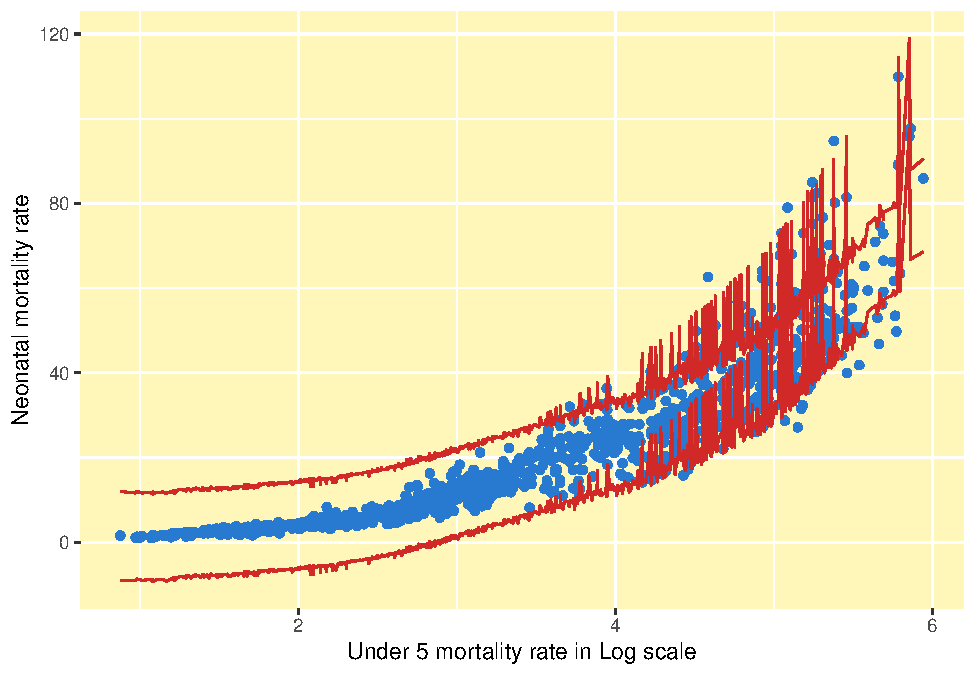
\includegraphics{A2_files/figure-latex/unnamed-chunk-19-1.pdf}

\begin{Shaded}
\begin{Highlighting}[]
\NormalTok{augment\_non\_linear }\SpecialCharTok{\%\textgreater{}\%} 
  \FunctionTok{filter}\NormalTok{(country\_name }\SpecialCharTok{\%in\%} \FunctionTok{c}\NormalTok{(}\StringTok{"India"}\NormalTok{, }\StringTok{"Japan"}\NormalTok{, }\StringTok{"Australia"}\NormalTok{)) }\SpecialCharTok{\%\textgreater{}\%} 
  \FunctionTok{ggplot}\NormalTok{(}\FunctionTok{aes}\NormalTok{(}\AttributeTok{sample=}\NormalTok{.resid}\SpecialCharTok{/}\NormalTok{.sigma)) }\SpecialCharTok{+}
  \FunctionTok{geom\_qq}\NormalTok{()}\SpecialCharTok{+}
  \FunctionTok{geom\_abline}\NormalTok{(}\AttributeTok{intercept=}\DecValTok{0}\NormalTok{, }\AttributeTok{slope =} \DecValTok{1}\NormalTok{) }\SpecialCharTok{+}
  \FunctionTok{facet\_wrap}\NormalTok{(}\SpecialCharTok{\textasciitilde{}}\NormalTok{country\_name, }\AttributeTok{scales =} \StringTok{"free"}\NormalTok{) }\SpecialCharTok{+}
  \FunctionTok{theme}\NormalTok{(}\AttributeTok{panel.background =} \FunctionTok{element\_rect}\NormalTok{(}\AttributeTok{fill =} \StringTok{"\#f0fcfc"}\NormalTok{),}
        \AttributeTok{plot.title =} \FunctionTok{element\_text}\NormalTok{(}\AttributeTok{hjust =} \FloatTok{0.5}\NormalTok{)) }\SpecialCharTok{+}
  \FunctionTok{ggtitle}\NormalTok{(}\StringTok{"QQ Plot for India, Japan, Australia in non{-}linear model"}\NormalTok{)}
\end{Highlighting}
\end{Shaded}

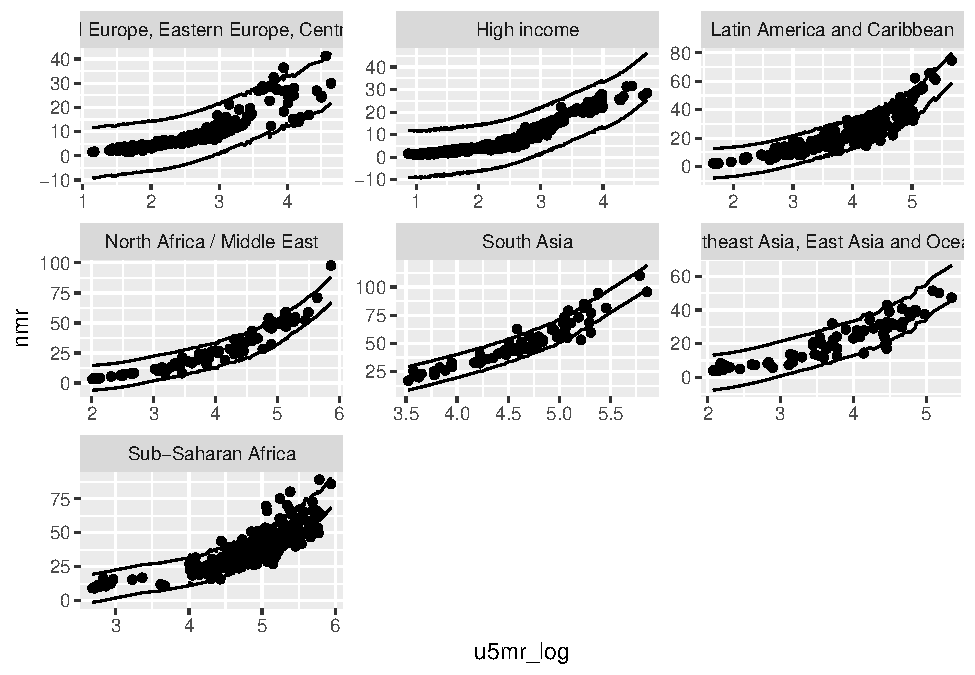
\includegraphics{A2_files/figure-latex/unnamed-chunk-19-2.pdf}

The non-linear model apparently fits better than the linear model for
Australia, India and Japan. Take Australia for example, the model
catches log\_u5mr around 2.0 to 2.5 better, most of the value at this
range are lower than others, and the fit model follows this trend while
it is the opposite for the linear model. The predicted values differ
largely from the observed values as shown in the QQ-Plot, as there are
clearly some violations.

\hypertarget{task-1.2.4-estimate-the-root-mean-square-error-and-the-mean-absolute-error-using-the-same-test-set-as-before.}{%
\subsubsection{Task 1.2.4: Estimate the root mean square error and the
mean absolute error using the same test set as
before.}\label{task-1.2.4-estimate-the-root-mean-square-error-and-the-mean-absolute-error-using-the-same-test-set-as-before.}}

\begin{Shaded}
\begin{Highlighting}[]
\CommentTok{\# Predict the test dataset}
\NormalTok{lm\_pred }\OtherTok{\textless{}{-}} \FunctionTok{tibble}\NormalTok{(}\AttributeTok{pred =} \FunctionTok{predict}\NormalTok{(fit\_non\_linear, nmr\_test))}
\NormalTok{lm\_pred }\OtherTok{\textless{}{-}} \FunctionTok{bind\_cols}\NormalTok{(nmr\_test, lm\_pred)}
\NormalTok{lm\_pred }\SpecialCharTok{\%\textgreater{}\%} 
  \FunctionTok{metrics}\NormalTok{(}\AttributeTok{truth =}\NormalTok{ transformed\_nmr,}
          \AttributeTok{estimate =}\NormalTok{ pred) }\SpecialCharTok{\%\textgreater{}\%} 
  \FunctionTok{kbl}\NormalTok{(}\AttributeTok{booktabs =}\NormalTok{ T) }\SpecialCharTok{\%\textgreater{}\%}
  \FunctionTok{kable\_styling}\NormalTok{(}\AttributeTok{position =} \StringTok{"center"}\NormalTok{)}
\end{Highlighting}
\end{Shaded}

\begin{table}
\centering
\begin{tabular}[t]{llr}
\toprule
.metric & .estimator & .estimate\\
\midrule
rmse & standard & 0.41\\
rsq & standard & 0.62\\
mae & standard & 0.28\\
\bottomrule
\end{tabular}
\end{table}

\hypertarget{task-1.2.5-produce-a-prediction-with-prediction-intervals8-of-the-nmr-on-its-natural-scale-aka-not-on-the-log-scale-and-plot-these-a-for-all-data-simultaneously-b-for-data-in-each-region-and-c-for-data-in-a-maximum-of-3-countries-that-show-different-aspects-of-the-fit.}{%
\subsubsection{Task 1.2.5: Produce a prediction, with prediction
intervals8, of the NMR on its natural scale (aka not on the log-scale)
and plot these a) for all data simultaneously; b) for data in each
region; and c) for data in a maximum of 3 countries that show different
aspects of the
fit.}\label{task-1.2.5-produce-a-prediction-with-prediction-intervals8-of-the-nmr-on-its-natural-scale-aka-not-on-the-log-scale-and-plot-these-a-for-all-data-simultaneously-b-for-data-in-each-region-and-c-for-data-in-a-maximum-of-3-countries-that-show-different-aspects-of-the-fit.}}

\begin{Shaded}
\begin{Highlighting}[]
\NormalTok{fit\_non\_linear\_natural }\OtherTok{\textless{}{-}} \FunctionTok{lm}\NormalTok{(nmr }\SpecialCharTok{\textasciitilde{}} \FunctionTok{bs}\NormalTok{(u5mr\_log, }\AttributeTok{df=} \DecValTok{15}\NormalTok{) }\SpecialCharTok{+}\NormalTok{ u5mr\_log}\SpecialCharTok{*}\NormalTok{region }\SpecialCharTok{+}\NormalTok{ u5mr\_log}\SpecialCharTok{*}\NormalTok{time, }\AttributeTok{data =}\NormalTok{ nmr\_train)}
\CommentTok{\# Prediction for all data simultaneously}
\NormalTok{non\_linear\_prediction }\OtherTok{\textless{}{-}} \FunctionTok{as\_tibble}\NormalTok{(}\FunctionTok{predict}\NormalTok{(fit\_non\_linear\_natural, nmr\_test, }\AttributeTok{interval =} \StringTok{"prediction"}\NormalTok{)) }\SpecialCharTok{\%\textgreater{}\%} 
  \FunctionTok{bind\_cols}\NormalTok{(lm\_pred)}

\NormalTok{non\_linear\_prediction }\SpecialCharTok{\%\textgreater{}\%} 
  \FunctionTok{ggplot}\NormalTok{(}\FunctionTok{aes}\NormalTok{(}\AttributeTok{x =}\NormalTok{ u5mr\_log, }\AttributeTok{y =}\NormalTok{ nmr))}\SpecialCharTok{+}
  \FunctionTok{geom\_point}\NormalTok{(}\AttributeTok{color =} \StringTok{"\#287ad1"}\NormalTok{)}\SpecialCharTok{+}
  \FunctionTok{geom\_line}\NormalTok{(}\FunctionTok{aes}\NormalTok{(}\AttributeTok{y =}\NormalTok{ lwr), }\AttributeTok{color =} \StringTok{"\#d12828"}\NormalTok{)}\SpecialCharTok{+}
  \FunctionTok{geom\_line}\NormalTok{(}\FunctionTok{aes}\NormalTok{(}\AttributeTok{y =}\NormalTok{ upr), }\AttributeTok{color =} \StringTok{"\#d12828"}\NormalTok{) }\SpecialCharTok{+}
  \FunctionTok{theme}\NormalTok{(}\AttributeTok{panel.background =} \FunctionTok{element\_rect}\NormalTok{(}\AttributeTok{fill =} \StringTok{"\#fff6ba"}\NormalTok{)) }\SpecialCharTok{+}
  \FunctionTok{xlab}\NormalTok{(}\StringTok{"Under 5 mortality rate in Log scale"}\NormalTok{) }\SpecialCharTok{+}
  \FunctionTok{ylab}\NormalTok{(}\StringTok{"Neonatal mortality rate"}\NormalTok{)}
\end{Highlighting}
\end{Shaded}

\includegraphics{A2_files/figure-latex/unnamed-chunk-21-1.pdf}

\begin{Shaded}
\begin{Highlighting}[]
\CommentTok{\#  Prediction for region}
\NormalTok{non\_linear\_prediction }\SpecialCharTok{\%\textgreater{}\%}
  \FunctionTok{ggplot}\NormalTok{(}\FunctionTok{aes}\NormalTok{(}\AttributeTok{x =}\NormalTok{ u5mr\_log, }\AttributeTok{y =}\NormalTok{ nmr))}\SpecialCharTok{+}
  \FunctionTok{geom\_point}\NormalTok{(}\AttributeTok{color =} \StringTok{"\#287ad1"}\NormalTok{)}\SpecialCharTok{+}
  \FunctionTok{geom\_line}\NormalTok{(}\FunctionTok{aes}\NormalTok{(}\AttributeTok{y =}\NormalTok{ lwr), }\AttributeTok{color =} \StringTok{"\#d12828"}\NormalTok{) }\SpecialCharTok{+}
  \FunctionTok{geom\_line}\NormalTok{(}\FunctionTok{aes}\NormalTok{(}\AttributeTok{y =}\NormalTok{ upr), }\AttributeTok{color =} \StringTok{"\#d12828"}\NormalTok{)}\SpecialCharTok{+}
  \FunctionTok{facet\_wrap}\NormalTok{(}\SpecialCharTok{\textasciitilde{}}\NormalTok{ region, }\AttributeTok{scale =} \StringTok{"free"}\NormalTok{)}\SpecialCharTok{+}
  \FunctionTok{theme}\NormalTok{(}\AttributeTok{panel.background =} \FunctionTok{element\_rect}\NormalTok{(}\AttributeTok{fill =} \StringTok{"\#fff6ba"}\NormalTok{)) }\SpecialCharTok{+}
  \FunctionTok{xlab}\NormalTok{(}\StringTok{"Under 5 mortality rate in Log scale"}\NormalTok{) }\SpecialCharTok{+}
  \FunctionTok{ylab}\NormalTok{(}\StringTok{"Neonatal mortality rate"}\NormalTok{)}
\end{Highlighting}
\end{Shaded}

\includegraphics{A2_files/figure-latex/unnamed-chunk-21-2.pdf}

\begin{Shaded}
\begin{Highlighting}[]
\CommentTok{\#  Prediction for 3 Countires}
\NormalTok{ non\_linear\_prediction }\SpecialCharTok{\%\textgreater{}\%}
  \FunctionTok{filter}\NormalTok{(country\_name }\SpecialCharTok{\%in\%} \FunctionTok{c}\NormalTok{(}\StringTok{"India"}\NormalTok{, }\StringTok{"Japan"}\NormalTok{, }\StringTok{"Australia"}\NormalTok{)) }\SpecialCharTok{\%\textgreater{}\%} 
  \FunctionTok{ggplot}\NormalTok{(}\FunctionTok{aes}\NormalTok{(}\AttributeTok{x =}\NormalTok{ u5mr\_log, }\AttributeTok{y =}\NormalTok{ nmr))}\SpecialCharTok{+}
  \FunctionTok{geom\_point}\NormalTok{(}\AttributeTok{color =} \StringTok{"\#287ad1"}\NormalTok{)}\SpecialCharTok{+}
  \FunctionTok{geom\_line}\NormalTok{(}\FunctionTok{aes}\NormalTok{(}\AttributeTok{y =}\NormalTok{ lwr), }\AttributeTok{color =} \StringTok{"\#d12828"}\NormalTok{) }\SpecialCharTok{+}
  \FunctionTok{geom\_line}\NormalTok{(}\FunctionTok{aes}\NormalTok{(}\AttributeTok{y =}\NormalTok{ upr), }\AttributeTok{color =} \StringTok{"\#d12828"}\NormalTok{)}\SpecialCharTok{+}
  \FunctionTok{facet\_wrap}\NormalTok{(}\SpecialCharTok{\textasciitilde{}}\NormalTok{ country\_name, }\AttributeTok{scale =} \StringTok{"free"}\NormalTok{)}\SpecialCharTok{+}
  \FunctionTok{theme}\NormalTok{(}\AttributeTok{panel.background =} \FunctionTok{element\_rect}\NormalTok{(}\AttributeTok{fill =} \StringTok{"\#fff6ba"}\NormalTok{)) }\SpecialCharTok{+}
  \FunctionTok{xlab}\NormalTok{(}\StringTok{"Under 5 mortality rate in Log scale"}\NormalTok{) }\SpecialCharTok{+}
  \FunctionTok{ylab}\NormalTok{(}\StringTok{"Neonatal mortality rate"}\NormalTok{)}
\end{Highlighting}
\end{Shaded}

\includegraphics{A2_files/figure-latex/unnamed-chunk-21-3.pdf}

\hypertarget{conclusion-for-task-1}{%
\subsection{Conclusion for Task 1:}\label{conclusion-for-task-1}}

The first model is the linear regression model and second is the
non-linear regression model. The MAE and the RMSE are significant, which
means the errors of the predicted model cannot be ignored. The
non-linear model is more appropriate model to explain the data. However,
the R-squared value of the linear model and the non-linear model do not
show much difference indicating that the transformed\_nmr, u5mr\_log,
region and time variables are not highly dependent on each other. From
the graph of the model and qq plots, especially from for each region and
the three different countries, non-linear model have better fit over the
linear model.

\hypertarget{task-2-the-residual-bootstrap}{%
\section{Task 2: The residual
bootstrap}\label{task-2-the-residual-bootstrap}}

\hypertarget{introduction-1}{%
\subsection{Introduction:}\label{introduction-1}}

In this section we wrote a function that uses the residual bootstrap to
compute an 80\% confidence interval for the LASSO estimate for each
regression parameters also check the coverage of each of the intervals.

\begin{Shaded}
\begin{Highlighting}[]
\CommentTok{\#data}
\FunctionTok{set.seed}\NormalTok{(}\DecValTok{123}\NormalTok{)}

\NormalTok{p }\OtherTok{\textless{}{-}} \DecValTok{14}
\NormalTok{n }\OtherTok{\textless{}{-}} \DecValTok{10000}
\NormalTok{n\_sim }\OtherTok{\textless{}{-}} \DecValTok{10}

\NormalTok{data }\OtherTok{\textless{}{-}} \FunctionTok{matrix}\NormalTok{(}\FunctionTok{rnorm}\NormalTok{(n}\SpecialCharTok{*}\NormalTok{p), }\AttributeTok{nrow =}\NormalTok{ n, }\AttributeTok{ncol =}\NormalTok{ p) }\SpecialCharTok{\%\textgreater{}\%} 
  \FunctionTok{as\_tibble}\NormalTok{() }\SpecialCharTok{\%\textgreater{}\%} 
  \FunctionTok{mutate}\NormalTok{(}\AttributeTok{y =}\NormalTok{V1}\SpecialCharTok{+}\DecValTok{2}\SpecialCharTok{*}\NormalTok{V2}\DecValTok{{-}3}\SpecialCharTok{*}\NormalTok{V3}\SpecialCharTok{+}\NormalTok{V4}\SpecialCharTok{+}\FunctionTok{rnorm}\NormalTok{(n, }\AttributeTok{sd =} \FloatTok{0.4}\NormalTok{))}

\NormalTok{variables }\OtherTok{\textless{}{-}} \FunctionTok{paste0}\NormalTok{(}\StringTok{"V"}\NormalTok{, }\DecValTok{1}\SpecialCharTok{:}\DecValTok{14}\NormalTok{)}
\NormalTok{formula }\OtherTok{\textless{}{-}} \FunctionTok{reformulate}\NormalTok{(variables, }\AttributeTok{response =} \StringTok{"y"}\NormalTok{)}
\end{Highlighting}
\end{Shaded}

\hypertarget{write-a-function-that-uses-a-residual-bootstrap-to-compute-an-80-confidence-interval-for-the-lasso-estimate-for-each-regression-parameters.}{%
\subsection{Write a function that uses a residual bootstrap to compute
an 80\% confidence interval for the LASSO estimate for each regression
parameters.}\label{write-a-function-that-uses-a-residual-bootstrap-to-compute-an-80-confidence-interval-for-the-lasso-estimate-for-each-regression-parameters.}}

\begin{Shaded}
\begin{Highlighting}[]
\CommentTok{\# write the function}
\FunctionTok{library}\NormalTok{(glmnet)}

\NormalTok{lasso}\OtherTok{\textless{}{-}} \ControlFlowTok{function}\NormalTok{(data, formula, n, n\_sim)\{}
  
\CommentTok{\# model with tune to find a good value of the penalty parameter}
\NormalTok{  spec\_lasso\_tune }\OtherTok{\textless{}{-}} \FunctionTok{linear\_reg}\NormalTok{(}\AttributeTok{penalty =} \FunctionTok{tune}\NormalTok{(), }\AttributeTok{mixture =} \DecValTok{1}\NormalTok{) }\SpecialCharTok{\%\textgreater{}\%} 
    \FunctionTok{set\_engine}\NormalTok{(}\StringTok{"glmnet"}\NormalTok{)}
  
\NormalTok{  lambda\_grid }\OtherTok{\textless{}{-}} \FunctionTok{grid\_regular}\NormalTok{(}\FunctionTok{penalty}\NormalTok{(}\AttributeTok{range =} \FunctionTok{c}\NormalTok{(}\SpecialCharTok{{-}}\DecValTok{5}\NormalTok{,}\DecValTok{5}\NormalTok{)), }\AttributeTok{levels =} \DecValTok{10}\NormalTok{) }
  
\CommentTok{\#cross validation}
\NormalTok{  folds }\OtherTok{\textless{}{-}} \FunctionTok{vfold\_cv}\NormalTok{(data, }\AttributeTok{v =} \DecValTok{10}\NormalTok{) }

\CommentTok{\#workflow}
\NormalTok{  rec }\OtherTok{\textless{}{-}} \FunctionTok{recipe}\NormalTok{(formula, }\AttributeTok{data =}\NormalTok{ data)}

\NormalTok{  lasso\_wf }\OtherTok{\textless{}{-}} \FunctionTok{workflow}\NormalTok{() }\SpecialCharTok{\%\textgreater{}\%} 
    \FunctionTok{add\_recipe}\NormalTok{(rec) }\SpecialCharTok{\%\textgreater{}\%} 
    \FunctionTok{add\_model}\NormalTok{(spec\_lasso\_tune)}

\NormalTok{  lasso\_wf\_tune }\OtherTok{\textless{}{-}}\NormalTok{ lasso\_wf }\SpecialCharTok{\%\textgreater{}\%} 
    \FunctionTok{tune\_grid}\NormalTok{(}\AttributeTok{resamples =}\NormalTok{ folds,}
              \AttributeTok{grid =}\NormalTok{ lambda\_grid)}

\CommentTok{\#choose smallest mse }
\NormalTok{  smallest\_rmse }\OtherTok{\textless{}{-}}\NormalTok{ lasso\_wf\_tune }\SpecialCharTok{\%\textgreater{}\%} 
    \FunctionTok{select\_best}\NormalTok{(}\StringTok{"rmse"}\NormalTok{)}

\CommentTok{\#update lasso}
\NormalTok{  final\_lasso }\OtherTok{\textless{}{-}} \FunctionTok{finalize\_workflow}\NormalTok{(lasso\_wf, smallest\_rmse)}

\NormalTok{  fit\_lasso }\OtherTok{\textless{}{-}}\NormalTok{ final\_lasso }\SpecialCharTok{\%\textgreater{}\%} 
    \FunctionTok{fit}\NormalTok{(data)}

\CommentTok{\#Find intercept from v1 to v14 and predict estimate penality}
\NormalTok{  fit\_beta }\OtherTok{\textless{}{-}}\NormalTok{ final\_lasso }\SpecialCharTok{\%\textgreater{}\%} 
    \FunctionTok{fit}\NormalTok{(data) }\SpecialCharTok{\%\textgreater{}\%} 
    \FunctionTok{tidy}\NormalTok{()}

\CommentTok{\# compute residual (real {-} pred value)}
\NormalTok{  pred\_value }\OtherTok{\textless{}{-}}\NormalTok{ data }\SpecialCharTok{\%\textgreater{}\%} 
    \FunctionTok{bind\_cols}\NormalTok{(}\FunctionTok{predict}\NormalTok{(fit\_lasso, data))}

\NormalTok{  residuals }\OtherTok{\textless{}{-}}\NormalTok{ pred\_value }\SpecialCharTok{\%\textgreater{}\%} 
    \FunctionTok{summarise}\NormalTok{(}\AttributeTok{resid =}\NormalTok{ y }\SpecialCharTok{{-}}\NormalTok{ .pred)}

\CommentTok{\#Normalize the residuals}
\NormalTok{  normalized\_residuals }\OtherTok{\textless{}{-}}\NormalTok{ residuals }\SpecialCharTok{\%\textgreater{}\%} 
    \FunctionTok{summarise}\NormalTok{(}\AttributeTok{normalized\_resid =}\NormalTok{ resid }\SpecialCharTok{{-}} \FunctionTok{mean}\NormalTok{(resid))}

\CommentTok{\#Re{-}sample the residuals with replacement to create non{-}parametric bootstrap data}
\NormalTok{  np\_bs }\OtherTok{\textless{}{-}} \FunctionTok{tibble}\NormalTok{(}\AttributeTok{experiment =} \FunctionTok{rep}\NormalTok{(}\DecValTok{1}\SpecialCharTok{:}\NormalTok{n\_sim, }\AttributeTok{each =}\NormalTok{ n),}
                  \AttributeTok{index =} \FunctionTok{sample}\NormalTok{(}\DecValTok{1}\SpecialCharTok{:}\NormalTok{n, }\AttributeTok{size =}\NormalTok{ n}\SpecialCharTok{*}\NormalTok{n\_sim, }\AttributeTok{replace =} \ConstantTok{TRUE}\NormalTok{),}
                  \AttributeTok{resid\_star =}\NormalTok{ normalized\_residuals}\SpecialCharTok{$}\NormalTok{normalized\_resid[index],}
\NormalTok{                  pred\_value[index,]) }\SpecialCharTok{\%\textgreater{}\%}  \CommentTok{\# corresponding predict y value}
  \FunctionTok{mutate}\NormalTok{(}\AttributeTok{y\_hat =}\NormalTok{ .pred }\SpecialCharTok{+}\NormalTok{ resid\_star)}

\NormalTok{update\_rec }\OtherTok{\textless{}{-}} \FunctionTok{recipe}\NormalTok{(y\_hat }\SpecialCharTok{\textasciitilde{}}\NormalTok{ ., }\AttributeTok{data =}\NormalTok{ np\_bs[,}\SpecialCharTok{{-}}\DecValTok{1}\NormalTok{])}

\NormalTok{experiment }\OtherTok{\textless{}{-}}\NormalTok{  np\_bs }\SpecialCharTok{\%\textgreater{}\%} 
  \FunctionTok{group\_by}\NormalTok{(experiment) }\SpecialCharTok{\%\textgreater{}\%} 
  \FunctionTok{nest}\NormalTok{()}

\NormalTok{fit\_list }\OtherTok{\textless{}{-}} \FunctionTok{list}\NormalTok{()}

\CommentTok{\#Fit the LASSO to the bootstrap data}
  \ControlFlowTok{for}\NormalTok{ (i }\ControlFlowTok{in} \DecValTok{1}\SpecialCharTok{:}\FunctionTok{dim}\NormalTok{(experiment)[}\DecValTok{1}\NormalTok{])\{}
    
    \CommentTok{\#workflow}
\NormalTok{    updatde\_lasso\_wf }\OtherTok{\textless{}{-}} \FunctionTok{workflow}\NormalTok{() }\SpecialCharTok{\%\textgreater{}\%} 
    \FunctionTok{add\_recipe}\NormalTok{(update\_rec) }\SpecialCharTok{\%\textgreater{}\%} 
    \FunctionTok{add\_model}\NormalTok{(spec\_lasso\_tune)}

\NormalTok{    folds }\OtherTok{\textless{}{-}} \FunctionTok{vfold\_cv}\NormalTok{(experiment}\SpecialCharTok{$}\NormalTok{data[[i]], }\AttributeTok{v=} \DecValTok{10}\NormalTok{)}
  
\NormalTok{    lasso\_wf\_tune }\OtherTok{\textless{}{-}}\NormalTok{ updatde\_lasso\_wf}\SpecialCharTok{\%\textgreater{}\%} 
    \FunctionTok{tune\_grid}\NormalTok{(}\AttributeTok{resamples =}\NormalTok{ folds,}
            \AttributeTok{grid =}\NormalTok{ lambda\_grid)}
  
\NormalTok{    smallest\_rmse }\OtherTok{\textless{}{-}}\NormalTok{ lasso\_wf\_tune }\SpecialCharTok{\%\textgreater{}\%} 
    \FunctionTok{select\_best}\NormalTok{(}\StringTok{"rmse"}\NormalTok{)}

\NormalTok{  update\_final\_lasso }\OtherTok{\textless{}{-}} \FunctionTok{finalize\_workflow}\NormalTok{(updatde\_lasso\_wf, smallest\_rmse)}

\NormalTok{  fit\_list[[i]] }\OtherTok{\textless{}{-}}\NormalTok{ update\_final\_lasso }\SpecialCharTok{\%\textgreater{}\%} 
    \FunctionTok{fit}\NormalTok{(}\AttributeTok{data =}\NormalTok{ experiment}\SpecialCharTok{$}\NormalTok{data[[i]]) }\SpecialCharTok{\%\textgreater{}\%} 
    \FunctionTok{tidy}\NormalTok{() }\SpecialCharTok{\%\textgreater{}\%} 
    \FunctionTok{mutate}\NormalTok{(}\AttributeTok{exp =}\NormalTok{ i)}
\NormalTok{  \}}

\NormalTok{fit\_beta\_star }\OtherTok{\textless{}{-}} \FunctionTok{bind\_rows}\NormalTok{(fit\_list) }\SpecialCharTok{\%\textgreater{}\%} 
  \FunctionTok{rename}\NormalTok{(}\AttributeTok{bootstrap\_estimate =}\NormalTok{ estimate)}

\CommentTok{\#Compute the bias}
\NormalTok{bias }\OtherTok{\textless{}{-}}\NormalTok{ fit\_beta\_star }\SpecialCharTok{\%\textgreater{}\%} 
  \FunctionTok{group\_by}\NormalTok{(exp) }\SpecialCharTok{\%\textgreater{}\%} 
  \FunctionTok{mutate}\NormalTok{(}\AttributeTok{delta =}\NormalTok{ fit\_beta}\SpecialCharTok{$}\NormalTok{estimate }\SpecialCharTok{{-}}\NormalTok{ bootstrap\_estimate) }\SpecialCharTok{\%\textgreater{}\%} 
  \FunctionTok{left\_join}\NormalTok{(fit\_beta, }\AttributeTok{by =} \StringTok{"term"}\NormalTok{) }


\CommentTok{\#confidence interval}
\NormalTok{ci }\OtherTok{\textless{}{-}}\NormalTok{ bias }\SpecialCharTok{\%\textgreater{}\%} 
  \FunctionTok{group\_by}\NormalTok{(term) }\SpecialCharTok{\%\textgreater{}\%} 
  \FunctionTok{summarise}\NormalTok{(}\AttributeTok{lwr =}\NormalTok{ estimate }\SpecialCharTok{+}\FunctionTok{quantile}\NormalTok{(delta, }\FloatTok{0.1}\NormalTok{),}
            \AttributeTok{upr =}\NormalTok{ estimate }\SpecialCharTok{+}\FunctionTok{quantile}\NormalTok{(delta, }\FloatTok{0.9}\NormalTok{)) }\SpecialCharTok{\%\textgreater{}\%} 
  \FunctionTok{unique}\NormalTok{()}

\NormalTok{coverage }\OtherTok{\textless{}{-}}\NormalTok{ bias }\SpecialCharTok{\%\textgreater{}\%} 
  \FunctionTok{left\_join}\NormalTok{(ci, }\AttributeTok{by =} \StringTok{"term"}\NormalTok{) }\SpecialCharTok{\%\textgreater{}\%} 
  \FunctionTok{mutate}\NormalTok{(}\AttributeTok{covered =} \FunctionTok{ifelse}\NormalTok{(bootstrap\_estimate }\SpecialCharTok{\textgreater{}}\NormalTok{ lwr  }\SpecialCharTok{\&}\NormalTok{ bootstrap\_estimate }\SpecialCharTok{\textless{}}\NormalTok{ upr, }\DecValTok{1}\NormalTok{,}\DecValTok{0}\NormalTok{)) }\SpecialCharTok{\%\textgreater{}\%} 
  \FunctionTok{group\_by}\NormalTok{(term) }\SpecialCharTok{\%\textgreater{}\%} 
  \FunctionTok{summarise}\NormalTok{(}\AttributeTok{coverage =} \FunctionTok{mean}\NormalTok{(covered))}

\FunctionTok{return}\NormalTok{(}\FunctionTok{list}\NormalTok{(ci, coverage))}
\NormalTok{\}}
\end{Highlighting}
\end{Shaded}

\hypertarget{this-is-an-outcome-of-the-sample-data-of-80-confidence-interval-for-the-lasso-estimate}{%
\subsection{This is an outcome of the sample data of 80\% confidence
interval for the LASSO
estimate}\label{this-is-an-outcome-of-the-sample-data-of-80-confidence-interval-for-the-lasso-estimate}}

\begin{Shaded}
\begin{Highlighting}[]
\CommentTok{\# This is an outcome of the sample data of 80\% confidence interval  for the LASSO estimate}
\NormalTok{alist }\OtherTok{\textless{}{-}} \FunctionTok{lasso}\NormalTok{(data, formula, n, n\_sim) }

\NormalTok{ci }\OtherTok{\textless{}{-}}\NormalTok{ alist[}\DecValTok{1}\NormalTok{]}
\NormalTok{coverage }\OtherTok{\textless{}{-}}\NormalTok{ alist[}\DecValTok{2}\NormalTok{]}

\NormalTok{ci }\SpecialCharTok{\%\textgreater{}\%}
  \FunctionTok{kbl}\NormalTok{(}\AttributeTok{booktabs =}\NormalTok{ T,}
      \AttributeTok{caption =} \StringTok{"80\% confidence interval for Lasso"}\NormalTok{) }\SpecialCharTok{\%\textgreater{}\%}
  \FunctionTok{kable\_styling}\NormalTok{(}\AttributeTok{position =} \StringTok{"center"}\NormalTok{)}
\end{Highlighting}
\end{Shaded}

\textbackslash begin\{table\}
\textbackslash caption\{\label{tab:unnamed-chunk-24}80\% confidence
interval for Lasso\}

\begin{table}

\centering
\begin{tabular}[t]{lrr}
\toprule
term & lwr & upr\\
\midrule
.pred & NA & NA\\
(Intercept) & 0.00 & 0.00\\
index & NA & NA\\
resid\_star & NA & NA\\
V1 & -2.00 & -2.00\\
\addlinespace
V10 & 0.00 & 0.00\\
V11 & 0.00 & 0.00\\
V12 & 0.00 & 0.00\\
V13 & 0.00 & 0.00\\
V14 & 0.98 & 0.98\\
\addlinespace
V2 & 2.99 & 2.99\\
V3 & -2.98 & -2.98\\
V4 & 0.99 & 0.99\\
V5 & 0.00 & 0.00\\
V6 & 0.00 & 0.00\\
\addlinespace
V7 & 0.00 & 0.00\\
V8 & 0.00 & 0.00\\
V9 & 0.00 & 0.00\\
y & NA & NA\\
\bottomrule
\end{tabular}
\end{table}

\textbackslash end\{table\}

\hypertarget{write-a-function-that-checks-the-coverage-of-each-of-these-intervals-and-comment-on-whether-or-not-the-modified-residual-bootstrap-achieves-the-nominal-coverage}{%
\subsection{Write a function that checks the coverage of each of these
intervals and Comment on whether or not the (modified) residual
bootstrap achieves the nominal
coverage}\label{write-a-function-that-checks-the-coverage-of-each-of-these-intervals-and-comment-on-whether-or-not-the-modified-residual-bootstrap-achieves-the-nominal-coverage}}

\begin{Shaded}
\begin{Highlighting}[]
\NormalTok{coverage }\SpecialCharTok{\%\textgreater{}\%}
  \FunctionTok{kbl}\NormalTok{(}\AttributeTok{booktabs =}\NormalTok{ T,}
      \AttributeTok{caption =} \StringTok{"Coverage check for each interval"}\NormalTok{) }\SpecialCharTok{\%\textgreater{}\%}
  \FunctionTok{kable\_styling}\NormalTok{(}\AttributeTok{position =} \StringTok{"center"}\NormalTok{)}
\end{Highlighting}
\end{Shaded}

\begin{table}
\caption{\label{tab:unnamed-chunk-25}Coverage check for each interval}
\begin{table}

\centering
\begin{tabular}[t]{lr}
\toprule
term & coverage\\
\midrule
.pred & NA\\
(Intercept) & 0.1\\
index & NA\\
resid\_star & NA\\
V1 & 0.0\\
\addlinespace
V10 & 0.0\\
V11 & 0.0\\
V12 & 0.0\\
V13 & 0.0\\
V14 & 0.0\\
\addlinespace
V2 & 0.0\\
V3 & 0.0\\
V4 & 0.0\\
V5 & 0.0\\
V6 & 0.0\\
\addlinespace
V7 & 0.0\\
V8 & 0.0\\
V9 & 0.0\\
y & NA\\
\bottomrule
\end{tabular}
\end{table}
\end{table}

\hypertarget{conclusion-for-task-2}{%
\subsection{Conclusion for Task 2:}\label{conclusion-for-task-2}}

From the coverage table we can see that the modified residual bootstrap
does not achieve the nominal coverage.

\end{document}
